\documentclass[a4paper,14pt,oneside,openany]{memoir}

%%% Задаем поля, отступы и межстрочный интервал %%%

\usepackage[left=30mm, right=15mm, top=20mm, bottom=20mm]{geometry} % Пакет geometry с аргументами для определения полей
\pagestyle{plain} % Убираем стандарные для данного класса верхние колонтитулы с заголовком текущей главы, оставляем только номер страницы снизу по центру
\parindent=1.25cm % Абзацный отступ 1.25 см, приблизительно равно пяти знакам, как по ГОСТ
\usepackage{indentfirst} % Добавляем отступ к первому абзацу
%\linespread{1.3} % Межстрочный интервал (наиболее близко к вордовскому полуторному) - тут вместо этого используется команда OnehalfSpacing*

%%% Реализация библиографии пакетами biblatex и biblatex-gost с использованием движка biber %%%

\usepackage{csquotes} % Пакет для оформления сложных блоков цитирования (biblatex рекомендует его подключать)
\usepackage[
backend=biber,                                    
bibencoding=utf8,                                  
sorting=none,                                      
style=gost-numeric,                              
language=auto,                                    
autolang=other,                                    
sortcites=true,                            
movenames=false,                                  
maxnames=5,                                     
minnames=3,                                        
doi=false,                                   
isbn=false,                                      
]{biblatex}[2016/09/17]
\DeclareDelimFormat{bibinitdelim}{}                 % Убираем пробел между инициалами (Иванов И.И. вместо Иванов И. И.)
% Определяем файл с библиографией
\addbibresource{library.bib}  % Указываем путь к файлу библиографии (например, "library.bib")

%%% Задаем языковые параметры и шрифт %%%

\usepackage[english, russian]{babel}   % Настройки для русского языка как основного в тексте
\usepackage[nobreak]{hyphenat}
\babelfont{rm}{Times New Roman}                     % TMR в качестве базового roman-щрифта
\sloppy
\hyphenpenalty=10000
\exhyphenpenalty=10000
%%% Задаем стиль заголовков и подзаголовков в тексте %%%

\setsecnumdepth{subsection} % Номера разделов считать до третьего уровня включительно, т.е. нумеруются только главы, секции, подсекции
\renewcommand*{\chapterheadstart}{} % Переопределяем команду, задающую отступ над заголовком, чтобы отступа не было
\renewcommand*{\printchaptername}{} % Переопределяем команду, печатающую слово "Глава", чтобы оно не печалось
%\renewcommand*{\printchapternum}{} % То же самое для номера главы - тут не надо, номер главы оставляем
\renewcommand*{\chapnumfont}{\normalfont\bfseries} % Меняем стиль шрифта для номера главы: нормальный размер, полужирный
\renewcommand*{\afterchapternum}{\hspace{1em}} % Меняем разделитель между номером главы и названием
\renewcommand*{\printchaptertitle}{\normalfont\bfseries\centering\MakeUppercase} % Меняем стиль написания для заголовка главы: нормальный размер, полужирный, центрированный, заглавными буквами
\setbeforesecskip{20pt} % Задаем отступ перед заголовком секции
\setaftersecskip{20pt} % Ставим такой же отступ после заголовка секции
\setsecheadstyle{\raggedright\normalfont\bfseries} % Меняем стиль написания для заголовка секции: выравнивание по правому краю без переносов, нормальный размер, полужирный
\setbeforesubsecskip{20pt} % Задаем отступ перед заголовком подсекции
\setaftersubsecskip{20pt} % Ставим такой же отступ после заголовка подсекции
\setsubsecheadstyle{\raggedright\normalfont\bfseries}  % Меняем стиль написания для заголовка подсекции: выравнивание по правому краю без переносов, нормальный размер, полужирный

%%% Задаем параметры оглавления %%%

\addto\captionsrussian{\renewcommand\contentsname{Содержание}} % Меняем слово "Оглавление" на "Содержание"
\setrmarg{2.55em plus1fil} % Запрещаем переносы слов в оглавлении
%\setlength{\cftbeforechapterskip}{0pt} % Эта команда убирает интервал между заголовками глав - тут не надо, так красивее смотрится
\renewcommand{\aftertoctitle}{\afterchaptertitle \vspace{-\cftbeforechapterskip}} % Делаем отступ между словом "Содержание" и первой строкой таким же, как у заголовков глав
%\renewcommand*{\chapternumberline}[1]{} % Делаем так, чтобы номер главы не печатался - тут не надо
\renewcommand*{\cftchapternumwidth}{1.5em} % Ставим подходящий по размеру разделитель между номером главы и самим заголовком
\renewcommand*{\cftchapterfont}{\normalfont\MakeUppercase} % Названия глав обычным шрифтом заглавными буквами
\renewcommand*{\cftchapterpagefont}{\normalfont} % Номера страниц обычным шрифтом
\renewcommand*{\cftchapterdotsep}{\cftdotsep} % Делаем точки до номера страницы после названий глав
\renewcommand*{\cftdotsep}{1} % Задаем расстояние между точками
\renewcommand*{\cftchapterleader}{\cftdotfill{\cftchapterdotsep}} % Делаем точки стандартной формы (по умолчанию они "жирные")
\maxtocdepth{subsection} % В оглавление попадают только разделы первыхтрех уровней: главы, секции и подсекции

%%% Выравнивание и переносы %%%

%% http://tex.stackexchange.com/questions/241343/what-is-the-meaning-of-fussy-sloppy-emergencystretch-tolerance-hbadness
%% http://www.latex-community.org/forum/viewtopic.php?p=70342#p70342
\tolerance 1414
\hbadness 1414
\emergencystretch 1.5em                             % В случае проблем регулировать в первую очередь
\hfuzz 0.3pt
\vfuzz \hfuzz
%\dbottom
%\sloppy                                            % Избавляемся от переполнений
\clubpenalty=10000                                  % Запрещаем разрыв страницы после первой строки абзаца
\widowpenalty=10000                                 % Запрещаем разрыв страницы после последней строки абзаца
\brokenpenalty=4991                                 % Ограничение на разрыв страницы, если строка заканчивается переносом

%%% Объясняем компилятору, какие буквы русского алфавита можно использовать в перечислениях (подрисунках и нумерованных списках) %%%
%%% По ГОСТ нельзя использовать буквы ё, з, й, о, ч, ь, ы, ъ %%%
%%% Здесь также переопределены заглавные буквы, хотя в принципе они в документе не используются %%%

\makeatletter
    \def\russian@Alph#1{\ifcase#1\or
       А\or Б\or В\or Г\or Д\or Е\or Ж\or
       И\or К\or Л\or М\or Н\or
       П\or Р\or С\or Т\or У\or Ф\or Х\or
       Ц\or Ш\or Щ\or Э\or Ю\or Я\else\xpg@ill@value{#1}{russian@Alph}\fi}
    \def\russian@alph#1{\ifcase#1\or
       а\or б\or в\or г\or д\or е\or ж\or
       и\or к\or л\or м\or н\or
       п\or р\or с\or т\or у\or ф\or х\or
       ц\or ш\or щ\or э\or ю\or я\else\xpg@ill@value{#1}{russian@alph}\fi}
\makeatother

%%% Задаем параметры оформления рисунков и таблиц %%%

\usepackage{graphicx, caption, subcaption} % Подгружаем пакеты для работы с графикой и настройки подписей
\graphicspath{{images/}} % Определяем папку с рисунками
\captionsetup[figure]{font=small, width=\textwidth, name=Рисунок, justification=centering} % Задаем параметры подписей к рисункам: маленький шрифт (в данном случае 12pt), ширина равна ширине текста, полнотекстовая надпись "Рисунок", выравнивание по центру
\captionsetup[subfigure]{font=small} % Индексы подрисунков а), б) и так далее тоже шрифтом 12pt (по умолчанию делает еще меньше)
\captionsetup[table]{singlelinecheck=false,font=small,width=\textwidth,justification=justified} % Задаем параметры подписей к таблицам: запрещаем переносы, маленький шрифт (в данном случае 12pt), ширина равна ширине текста, выравнивание по ширине
\captiondelim{ --- } % Разделителем между номером рисунка/таблицы и текстом в подписи является длинное тире
\setkeys{Gin}{width=\textwidth} % По умолчанию размер всех добавляемых рисунков будет подгоняться под ширину текста
\renewcommand{\thesubfigure}{\asbuk{subfigure}} % Нумерация подрисунков строчными буквами кириллицы
%\setlength{\abovecaptionskip}{0pt} % Отбивка над подписью - тут не меняем
%\setlength{\belowcaptionskip}{0pt} % Отбивка под подписью - тут не меняем
\usepackage[section]{placeins} % Объекты типа float (рисунки/таблицы) не вылезают за границы секциии, в которой они объявлены

%%% Задаем параметры ссылок и гиперссылок %%% 

\usepackage{hyperref}                               % Подгружаем нужный пакет
\hypersetup{
    colorlinks=true,                                % Все ссылки и гиперссылки цветные
    linktoc=all,                                    % В оглавлении ссылки подключатся для всех отображаемых уровней
    linktocpage=true,                               % Ссылка - только номер страницы, а не весь заголовок (так выглядит аккуратнее)
    linkcolor=red,                                  % Цвет ссылок и гиперссылок - красный
    citecolor=red                                   % Цвет цитировний - красный
}

%%% Настраиваем отображение списков %%%

\usepackage{enumitem}                               % Подгружаем пакет для гибкой настройки списков
\renewcommand*{\labelitemi}{\normalfont{--}}        % В ненумерованных списках для пунктов используем короткое тире
\makeatletter
    \AddEnumerateCounter{\asbuk}{\russian@alph}     % Объясняем пакету enumitem, как использовать asbuk
\makeatother
\renewcommand{\labelenumii}{\asbuk{enumii})}        % Кириллица для второго уровня нумерации
\renewcommand{\labelenumiii}{\arabic{enumiii})}     % Арабские цифры для третьего уровня нумерации
\setlist{noitemsep, leftmargin=*}                   % Убираем интервалы между пунками одного уровня в списке
\setlist[1]{labelindent=\parindent}                 % Отступ у пунктов списка равен абзацному отступу
\setlist[2]{leftmargin=\parindent}                  % Плюс еще один такой же отступ для следующего уровня
\setlist[3]{leftmargin=\parindent}                  % И еще один для третьего уровня

%%% Счетчики для нумерации объектов %%%

\counterwithout{figure}{chapter}                    % Сквозная нумерация рисунков по документу
\counterwithout{equation}{chapter}                  % Сквозная нумерация математических выражений по документу
\counterwithout{table}{chapter}                     % Сквозная нумерация таблиц по документу

\usepackage{csquotes} % Пакет для оформления сложных блоков цитирования (biblatex рекомендует его подключать)
       
%%% Скрипт, который автоматически подбирает язык (и, следовательно, формат) для каждой библиографической записи %%%
%%% Если в названии работы есть кириллица - меняем значение поля langid на russian %%%
%%% Все оставшиеся пустые места в поле langid заменяем на english %%%

\DeclareSourcemap{
  \maps[datatype=bibtex]{
    \map{
        \step[fieldsource=title, match=\regexp{^\P{Cyrillic}*\p{Cyrillic}.*}, final]
        \step[fieldset=langid, fieldvalue={russian}]
    }
    \map{
        \step[fieldset=langid, fieldvalue={english}]
    }
  }
}

\usepackage{amsmath}
\usepackage{gensymb}
\usepackage{wrapfig}

\usepackage{longtable,ltcaption}                    % Длинные таблицы
\usepackage{multirow,makecell}                      % Улучшенное форматирование таблиц
\usepackage{booktabs}                               % Еще один пакет для красивых таблиц
\usepackage{soulutf8}                               % Поддержка переносоустойчивых подчёркиваний и зачёркиваний
\usepackage{icomma}                                 % Запятая в десятичных дробях
\usepackage{hyphenat}                               % Для красивых переносов
\usepackage{textcomp}                               % Поддержка "сложных" печатных символов типа значков иены, копирайта и т.д.
\usepackage[version=4]{mhchem}                      % Красивые химические уравнения
\usepackage{amsmath}                                % Усовершенствование отображения математических выражений 

%%% Вставляем по очереди все содержательные части документа %%%

\begin{document}

\thispagestyle{empty}

\begin{center}
    МИНИСТЕРСТВО НАУКИ И ВЫСШЕГО ОБРАЗОВАНИЯ \\ РОССИЙСКОЙ ФЕДЕРАЦИИ

    \vspace{20pt}

    Федеральное государственное автономное \\ образовательное учреждение высшего образования \\
    «Национальный исследовательский ядерный университет “МИФИ”» 

    \vspace{20pt}

    {Научно-образовательный центр НЕВОД}
\end{center}

\vfill

\begin{center}
    ОТЧЕТ \\  
     о прохождении производственной практики \\ (научно-исследовательской работы)

    \vspace{20pt}

    \uppercase{«Поиск и анализ совместных событий 
на установках ДЕКОР и НЕВОД-ШАЛ»
}
\end{center}

\vfill
\hfill
\begin{flushright}
    \begin{tabular}{rl}
        Студент: & Альхимович М.Д. \\[0.5cm]
        Группа: & Б21-104 \\[0.5cm]
        Научный руководитель: & Богданов А.Г. \\
    \end{tabular}
\end{flushright}
\vfill

\begin{center}
    г. Москва\\
 2024
\end{center}                                     % Титульник

\newpage % Переходим на новую страницу
\setcounter{page}{2} % Начинаем считать номера страниц со второй
\OnehalfSpacing* % Задаем полуторный интервал текста (в титульнике одинарный, поэтому команда стоит после него)
\section*{Аннотация}
\label{ch:intro_ru}
	Научно-исследовательская работа посвящена поиску и анализу совместных событий на установках ДЕКОР И НЕВОД-ШАЛ. В рамках исследования были реализованы программные скрипты для поиска совместных событий, рассмотрены, реализованы и сравнены различные подходы реконструкции направления прихода широкого атмосферного ливня. 
	Результаты работы представлены в виде распределений числа событий по зенитному \(\theta\) и азимутальному \(\phi\) углу направлений прихода событий.
    
\section*{Abstract}
\label{ch:intro_en}
The research work is dedicated to the search and analysis of coincident events on the DECOR and NEVOD-EAS installations. As part of the study, software scripts were developed for detecting coincident events, and various approaches to reconstructing the arrival direction of extensive air showers were considered, implemented, and compared.
The results are presented as distributions of the number of events over the zenith angle \(\theta\) and the azimuthal angle \(\phi\)  of the event arrival directions.


\endinput  
\newpage
\tableofcontents*                                   % Автособираемое оглавление

\chapter*{Введение}
\addcontentsline{toc}{chapter}{Введение}
\label{ch:intro}

     В области энергий выше $10^{15}$ эВ интенсивность потока первичных космических лучей (ПКЛ) довольно мала, что делает затруднительным проведение прямых измерений их энергии и массового состава с помощью детекторов, размещенных на космических аппаратах или аэростатах. Поэтому единственным источником информации о свойствах первичных космических лучей в данной энергетической области на сегодняшний день являются широкие атмосферные ливни (ШАЛ), которые представляют собой ядерно-электромагнитные каскады, инициированные при взаимодействии первичных частиц с ядрами атомов воздуха.
     Уникальная научная установка «Экспериментальный комплекс НЕВОД» (ЭК НЕВОД), расположенная на территории НИЯУ МИФИ, позволяет проводить фундаментальные и прикладные исследования с использованием природных потоков частиц на поверхности Земли. 
     
	Одной из наиболее интересных задач ЭК НЕВОД является изучение групп мюонов, представляющих собой одновременное (в пределах десятков наносекунд) прохождение через установку проникающих частиц с практически параллельными треками, с помощью прецизионного трекового детектора ДЕКОР (проводится с 2002 г.) \cite{bogdanov2010investigation, kokoulin2021muon} и черенковского водного калориметра НЕВОД (с 2013 г.) \cite{yurina2021measurements}. Исследование мюонной компоненты ШАЛ в целом дает возможность получать информацию о массовом составе ПКЛ и проверять модели адронных взаимодействий при сверхвысоких энергиях. Функционирование в составе ЭК НЕВОД установки НЕВОД-ШАЛ поможет осуществить привязку событий с группами мюонов к традиционным методам регистрации ШАЛ, где определяется положение оси, мощность ливня, направление, и изучить, например, пространственное распределение мюонов.
    



\endinput                                     % Введение
\chapter*{Установка НЕВОД-ДЕКОР}
\addcontentsline{toc}{chapter}{Установка НЕВОД-ДЕКОР}
\label{ch:intro}

Координатно-трековый детектор ДЕКОР \cite{barbashina2000coordinate} представляет собой крупномасштабную установку, специально предназначенную для изучения мюонов космического излучения на поверхности Земли в широком диапазоне зенитных углов вплоть до горизонта. Установка состоит из 8 сборок-супермодулей (СМ00 – СМ07) по 8 слоев пластиковых камер из стримерных трубок, общая площадь ~ 70 м$^2$, 32768 каналов регистрации. По данным детектора ДЕКОР можно найти количество треков в группе мюонов и определить ее направление. Точность локализации трека в одном СМ лучше 1 см, а точность оценки направления – лучше $1\degree$. Супермодули детектора ДЕКОР расположены в галереях здания с трех сторон от черенковского водного детектора (ЧВД) НЕВОД объемом 2000 м$^3$. На рис. 1 изображена схема установки НЕВОД-ДЕКОР (а) и структура супермодуля детектора ДЕКОР (б).

\begin{figure}[ht]
	\centering
\hspace*{\fill}%
	\begin{subfigure}[b]{0.7\textwidth}
        \centering
		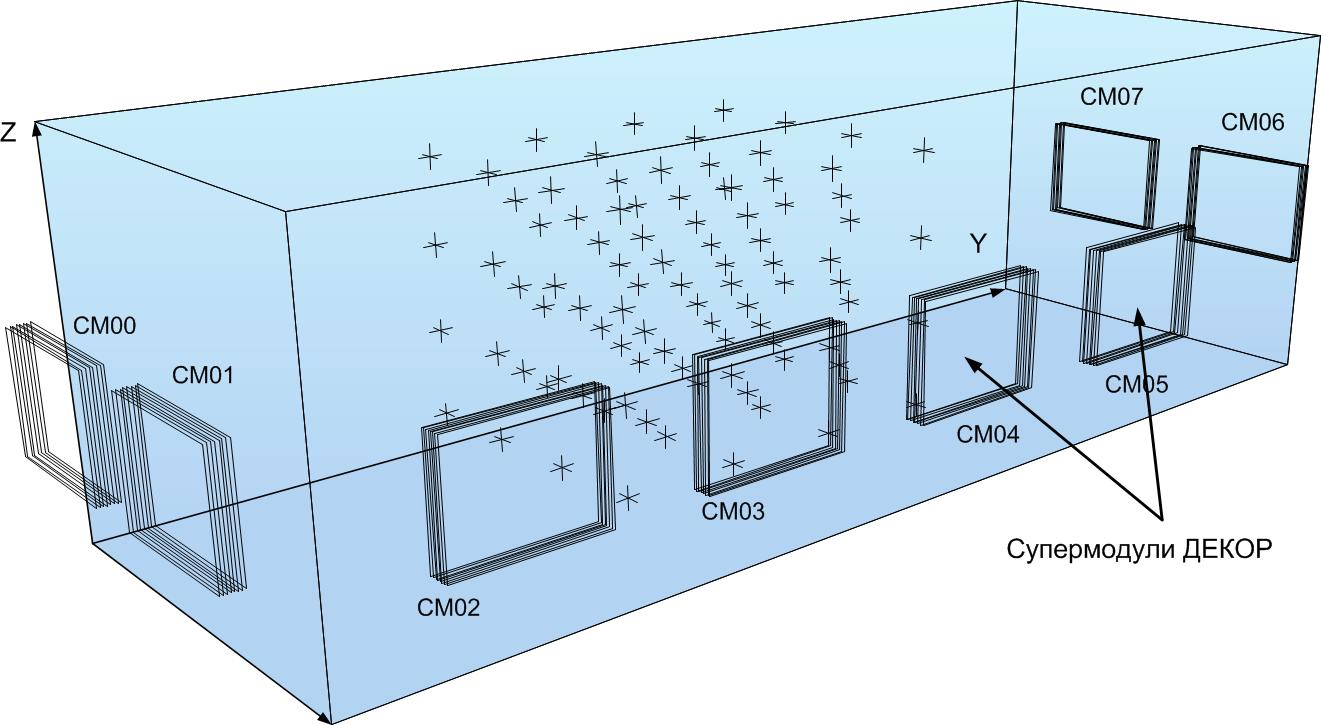
\includegraphics[height=10cm,keepaspectratio]{DECOR_1}
		\caption{}
		\label{fig:DECOR_1}
	\end{subfigure}
\hfill
	\begin{subfigure}[b]{0.29\textwidth}
        \centering
		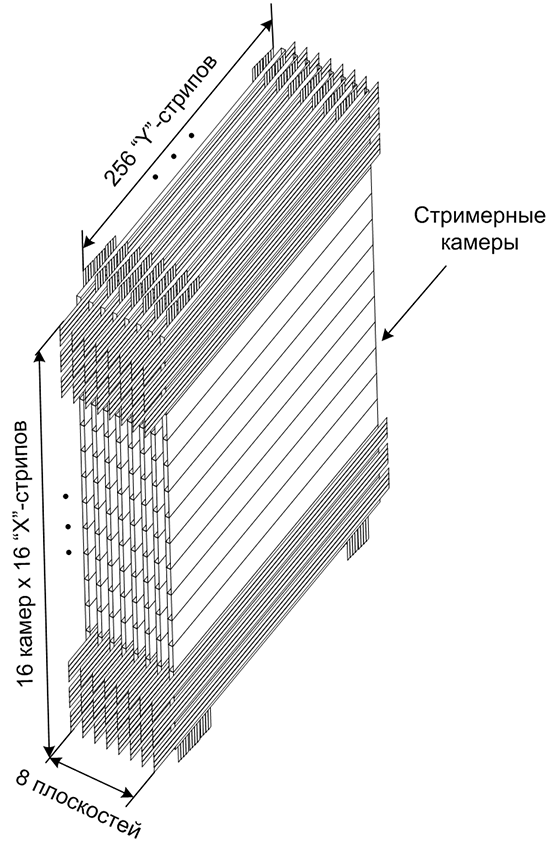
\includegraphics[height=10cm,keepaspectratio]{DECOR_2}
        \caption{}
		\label{fig:DECOR_2}
	\end{subfigure}
\hspace*{\fill}%
	\caption{Общая схема установки НЕВОД-ДЕКОР (a) и структура супермодуля детектора ДЕКОР (б)}
	\label{fig:tiger}
\end{figure}

НЕВОД \cite{petrukhin2015cherenkov} предназначен для изучения всех основных компонент космических лучей на поверхности Земли и состоит из 91 квазисферического измерительного модуля (КСМ), которые расположены в узлах пространственной решетки. Фактически решетка сформирована из 25 вертикальных гирлянд по 3 или 4 КСМ. Каждый КСМ состоит из 6 фотоумножителей с плоским фотокатодом, ориентированных вдоль осей ортогональной системы координат. Такая конструкция обеспечивает практически одинаковую эффективность регистрации черенковского излучения, приходящего с любого направления. Широкий динамический диапазон измерений каждого ФЭУ (от 1 до $10^5$ фотоэлектронов) позволяет проводить калориметрические исследования, в частности, измерять энерговыделения групп мюонов. 
Для калибровки спектрометрических трактов черенковского водного калориметра НЕВОД во время длительных экспериментальных серий, а также для исследований широких атмосферных
ливней энергетическом диапазоне первичных частиц от 0.1 до 100 ПэВ используется система калибровочных телескопов (СКТ). Система калибровочных телескопов (СКТ) состоит из 80 сцинтилляционных детекторов. Сорок детекторов расположены на крышке и сорок – на дне водного бассейна ЧВК НЕВОД (верхняя и нижняя плоскости).

\endinput                                 % НЕВОД ДЕКОР
\chapter*{Установка НЕВОД-ШАЛ}
\addcontentsline{toc}{chapter}{Установка НЕВОД-ШАЛ}
\label{ch:intro}

Установка НЕВОД-ШАЛ \cite{amelchakov2022nevod} предназначена для регистрации преимущественно электронно-фотонной компоненты широких атмосферных ливней в энергетическом диапазоне от $10^{15}$ до $10^{17}$ эВ. Её детектирующие элементы размещаются на крышах корпусов университета и на поверхности Земли (перепад высот достигает 20 м) на площади около $10^4$ м$^2$. Разновысотность расположения детектирующих элементов НЕВОД-ШАЛ определяет кластерную организацию ее регистрирующей системы. В состав установки НЕВОД-ШАЛ входит 9 кластеров по 4 детектирующих станции (ДС), расстояние между центрами соседних кластеров составляет около 30 м. Каждая станция состоит из 4 пластиковых сцинтилляционных счетчиков площадью $0.8 \times 0.8$ м$^2$ и толщиной 4 см, просматриваемых ФЭУ. При этом три счетчика оснащены одним фотоумножителем, а четвертый оборудован еще и дополнительным ФЭУ – для расширения динамического диапазона измерений до 10$^5$ частиц.

Каждый кластер оснащен своим локальным пунктом, который независимо осуществляет сбор и оцифровку аналоговых сигналов с детектирующих элементов, отбор событий по триггерным условиям, присваивание событиям временной метки и, таким образом, является самостоятельной ливневой установкой, способной определять как число частиц, зарегистрированных каждым детектирующим элементом, так и направление прихода фронта широких атмосферных ливней. 

На риcунке 2 изображена схема расположения кластеров установки НЕВОД-ШАЛ на территории НИЯУ МИФИ, а также конструкция счетчика и детектирующая станция. 

\begin{figure}[ht!]
    \centering
    % Первая большая картинка
    \subfloat[]{%
        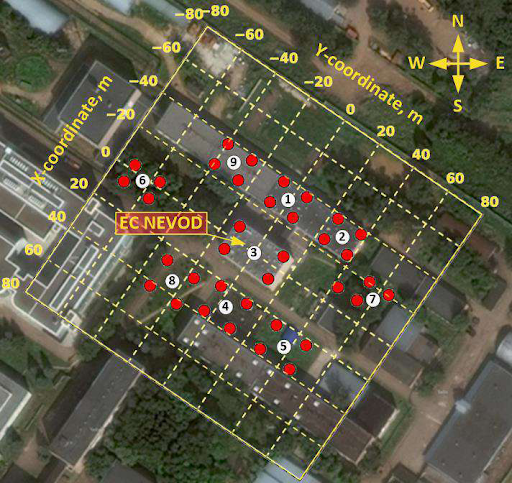
\includegraphics[width=0.95\textwidth, keepaspectratio]{images/невод-шал.png}%
        \label{fig:big_image}%
    }


    % Две маленькие картинки
    \subfloat[]{%
        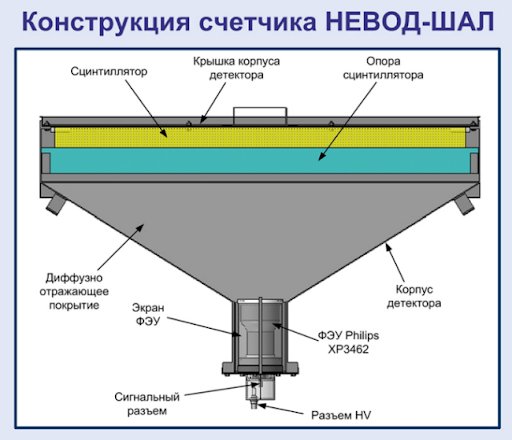
\includegraphics[height=5.2cm, keepaspectratio]{images/счетчик_шал.png}%
        \label{fig:small_image1}%
    }
    \hspace{0.04\textwidth}
    \subfloat[]{%
        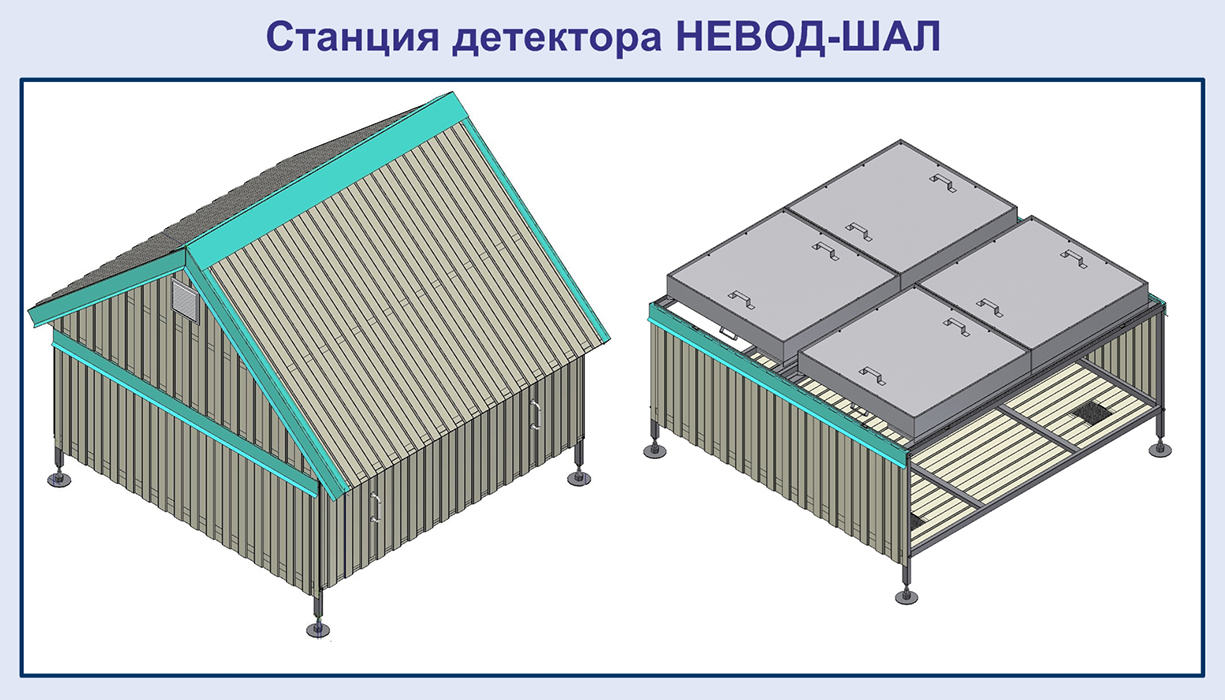
\includegraphics[height=5.2cm, keepaspectratio]{images/ds.jpg}%
        \label{fig:small_image2}%
    }

    \caption{Схема расположения кластеров установки НЕВОД-ШАЛ вокруг ЭК НЕВОД (a), конструкция счетчика (б) и детектирующая станция (a)}
    \label{fig:small_images}
\end{figure}


% Две маленькие картинки с текстом сверху и синей обводкой и тенью





\endinput                                 % НЕВОД ШАЛ
\chapter*{Система глобальной временной синхронизации (СГВС)}
\addcontentsline{toc}{chapter}{Система глобальной временной синхронизации (СГВС)}
\label{ch:intro}

Для обеспечения синхронной работы кластеров установки, а также привязки регистрируемых событий к мировому времени используется система глобальной временной синхронизации (СГВС) \cite{amelchakov2022nevod}. В состав СГВС входят: модуль глобальной временной синхронизации (МГВС), антенна GPS/ГЛОНАСС и управляющая ЭВМ. 

Основными функциями модуля МГВС являются:
\begin{itemize}
    \item раздача единой тактовой частоты 100 МГц в синхронизируемые устройства;
    \item раздача временных меток в синхронизируемые устройства для синхронного запуска их локальных часов;
    \item независимая синхронизация любого из каналов;
    \item синхронизация локальных часов реального времени с внешним приемником GPS;
    \item передача по сети Ethernet времени локальных часов и GPS-приемника.
\end{itemize}

Точность синхронизации локальных часов кластеров установки составляет 10 нс (1 период тактового генератора, установленного в модуле МГВС). Система СГВС применяется и для синхронизации локальных часов триггерной системы НЕВОД-ДЕКОР, работающей на собственной тактовой частоте 40 МГц. Для этого с выхода МГВС передается только временная метка. Точность синхронизации между НЕВОД-ШАЛ и НЕВОД-ДЕКОР при этом составляет около 25 нс.




\endinput                                  % Система глобальной временной
\chapter*{События с группами мюонов в детекторе ДЕКОР}
\addcontentsline{toc}{chapter}{События с группами мюонов в детекторе ДЕКОР}
\label{ch:intro}
Стандартный отбор и анализ групп мюонов по данным детектора ДЕКОР проводится для множественностей мюонов в группе \(m \geq 5\) и зенитных углов \(\theta \geq 55\degree\), чтобы исключить возможное влияние электронно-фотонной и адронной компонент ШАЛ на реконструкцию треков. Однако из части экспериментального материала в интервале зенитных углов \(40\degree \leq \theta < 55\degree\) (вследствие резкого увеличения статистики с уменьшением зенитного угла) операторами ЭК НЕВОД было отобрано 30 375 групп с множественностью мюонов \(m \leq 5\) (за 6 324 ч) и 4 139 групп с множественностью \(m = 4\) (за 1 043 ч). В этом случае установка НЕВОД-ШАЛ в принципе еще должна быть способна регистрировать электронно-фотонную компоненту ШАЛ, что позволяет провести анализ указанных событий совместно как минимум по двум компонентам ШАЛ. Отметим также, что события с группами мюонов отбирались в двух \(60\degree\) секторах азимутальных углов, где шесть из восьми СМ детектора ДЕКОР экранированы водным объемом детектора НЕВОД, причем во внимание принимаются данные только этих шести СМ. Пороговая энергия мюонов при этом составляет около 2 ГэВ. 

Отбор событий с умеренными зенитными углами проводился по 12-й серии измерений из наборов данных (RUN) 622-688 (с 15.02.18 по 29.05.18 г.) и 810-841 (с 13.12.18 по 03.02.19 г.). На рис. 3 изображен пример события с группой мюонов, зарегистрированного установкой ДЕКОР (a) и пространственной реконструкции треков (б).
\newpage
\noindent 19-12-2018 03:02:35.298.921.862, RUN \(=813\),  Event \(=73818\),\\
\(m = 9\), \(\theta = 41.9\degree\), \(\phi=204.9\degree\)

\begin{figure}[ht]
    \centering
    \subfloat[]{%
        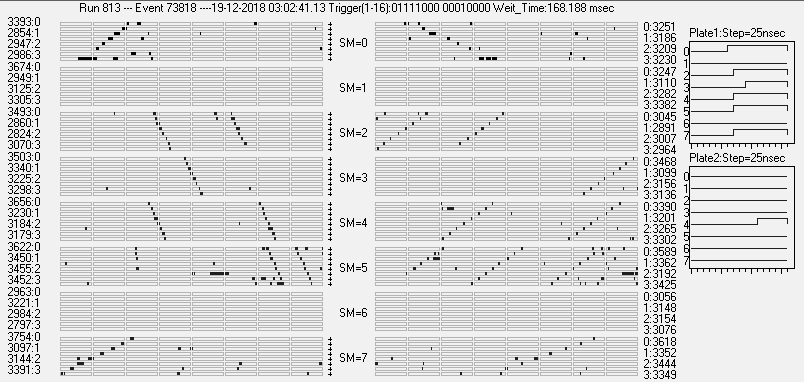
\includegraphics[width=0.95\textwidth, keepaspectratio]{images/73818_1_bw.png}%
        \label{fig:muon_group1}%
    }%

    \subfloat[]{%
        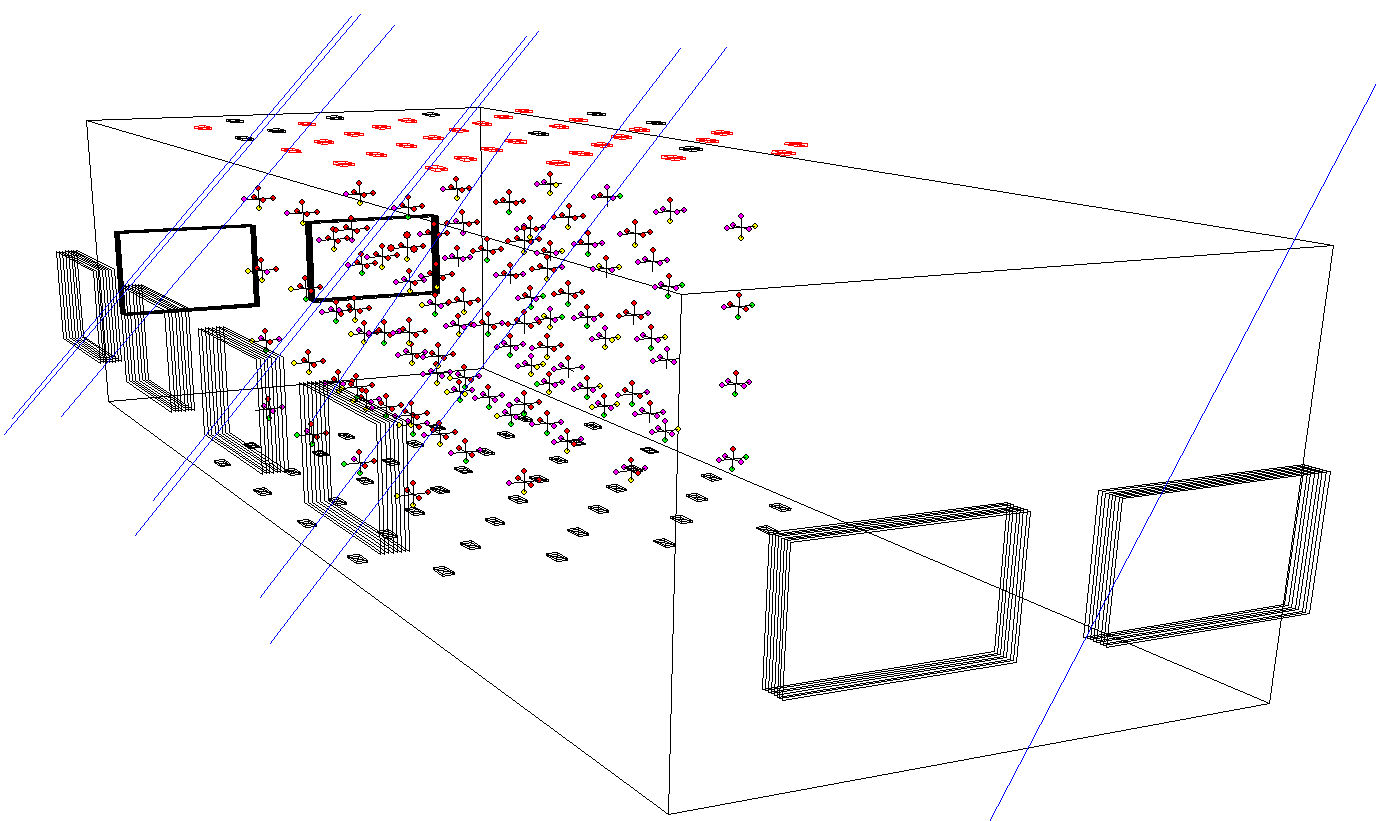
\includegraphics[width=0.95\textwidth, keepaspectratio]{images/73818.png}%
        \label{fig:muon_group}%
    }%

    \caption{Пример события с группой мюонов, зарегистрированного установкой \\ДЕКОР (a) и пространственной реконструкции треков (б)}
    \label{fig:muon_example}
\end{figure}

\newpage
На рисунке 4 представлено распределение зенитного \(\theta\) и азимутального \(\phi\) углов направления прихода 6990 отобранных групп мюонов 810-841 RUN

\begin{figure}[ht]
    \lefting
    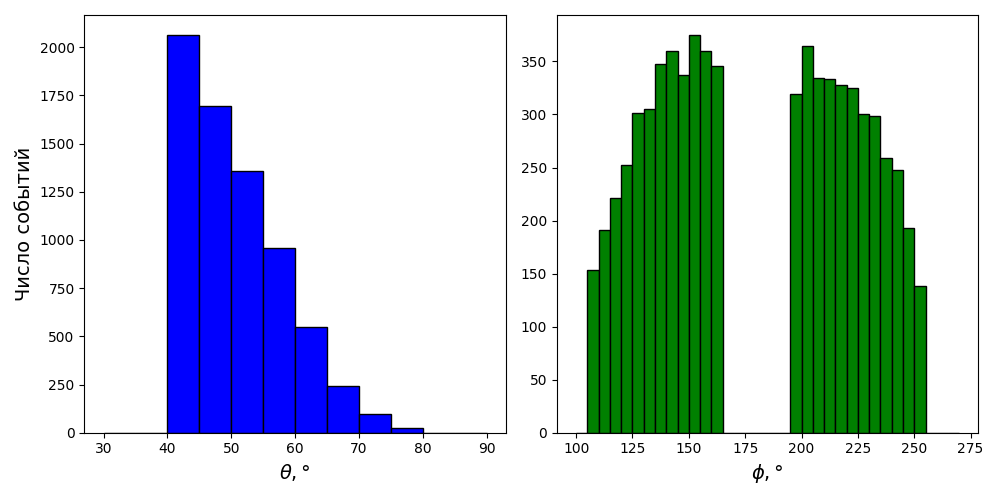
\includegraphics[width=1\textwidth]{images/theta_phi.png}
    \caption{Распределение числа событий с группами мюонов по зенитному\(\theta\) и азимутальному \(\phi\) углу направления прихода}
    \label{fig:phi_hist}
\end{figure}

\endinput                           % группы мюонов
\chapter*{Совместные события на установках ДЕКОР и НЕВОД-ШАЛ}
\addcontentsline{toc}{chapter}{Совместные события на установках ДЕКОР и НЕВОД-ШАЛ}
\label{ch:intro}
Были отобраны события, зарегистрированные на установках ДЕКОР и НЕВОД-ШАЛ за период с 19.12.2018 по 02.02.2019, в пределах временного интервала \(|\Delta t| = |t_{\text{Д}} - t_{\text{НШ}}|  < 1000\) нс, где 

\begin{itemize}
    \item \(t_{\text{Д}}\) время регистрации события ДЕКОР,
    \item \(t_{\text{НШ}}\) время регистрации события НЕВОД-ШАЛ.
\end{itemize}
Было найдено 5214 события. Создана база данных MongoDB найденных совместных событий установок. Среднее значение временного интервала составило \( \mu_t = 336.8 \) нс, а среднее отклонение \( \sigma = 52.8 \) нс. На рисунке 5 представлено распределение совместных событий по \(\Delta t\).
\begin{figure}[ht]
    \centering
    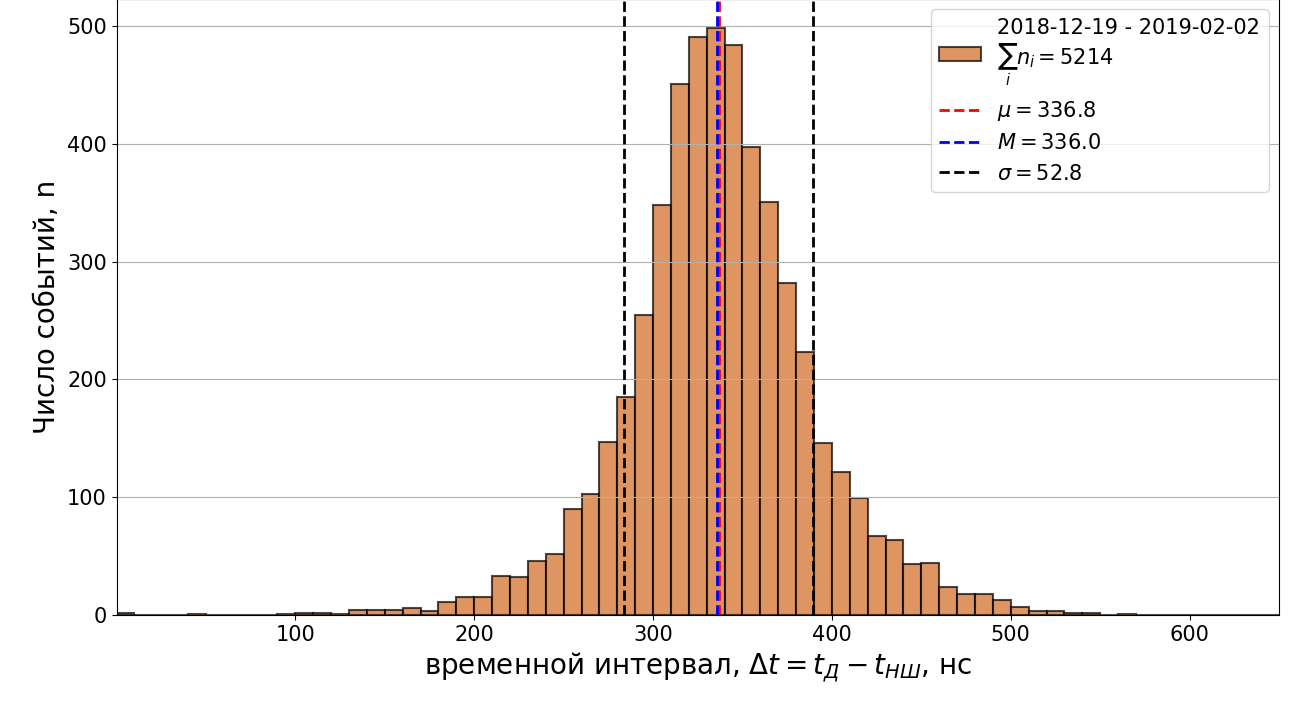
\includegraphics[width=0.9\textwidth]{images/events_by_delta_time.png}
    \caption{Распределение числа совместных событий по временному интервалу между событиями на установках ДЕКОР и НЕВОД-ШАЛ}
    \label{fig:your_image_label}
\end{figure}

Были определены совместные события с группами мюонов \(m > 5\). Распределение числа событий групп мюнов по номеру RUN и его длительности изображено на рисунке 6.

\begin{figure}[ht]
    \centering
    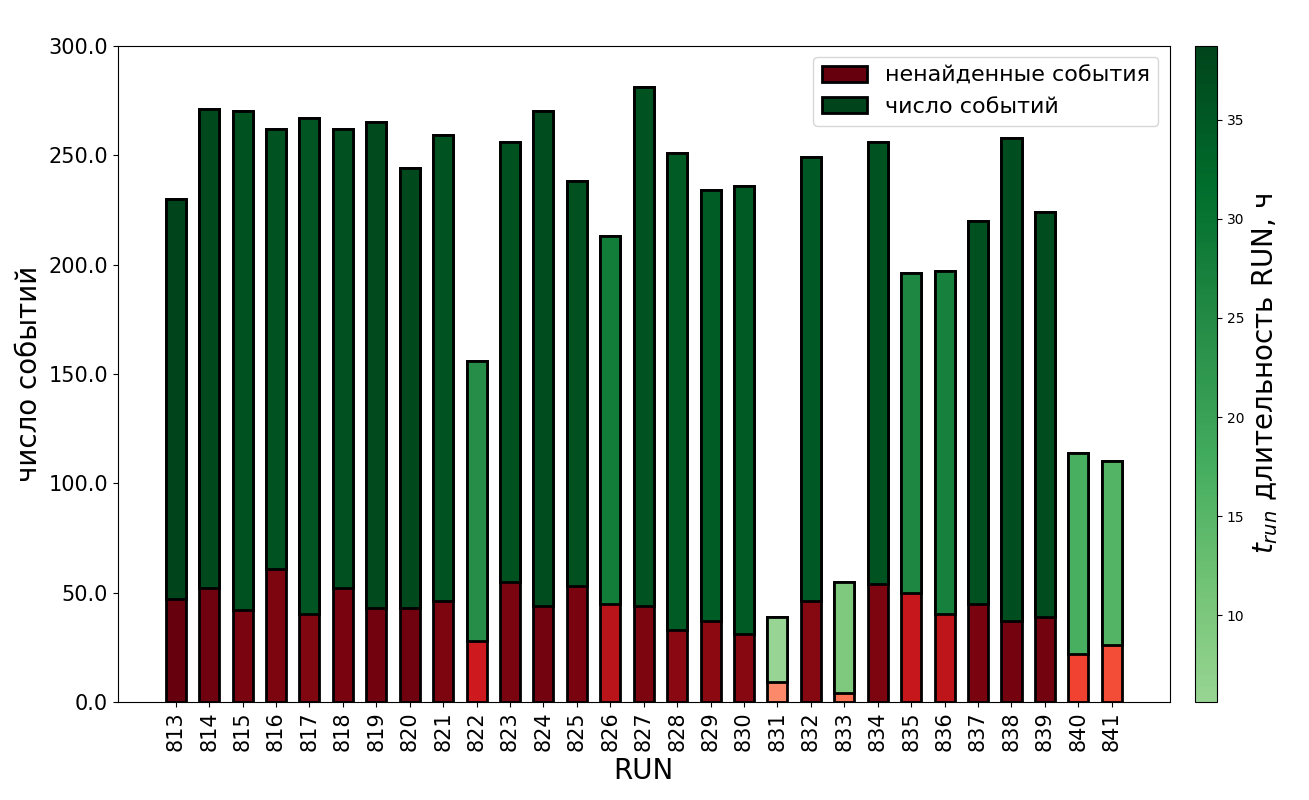
\includegraphics[width=0.9\textwidth]{images/muon_group_by_run.png}
    \caption{Распределение числа событий групп мюнов по номеру RUN}
    \label{fig:muon_group_by_run}
\end{figure}


\begin{figure}[h]
    \centering
    \subfloat[]{%
        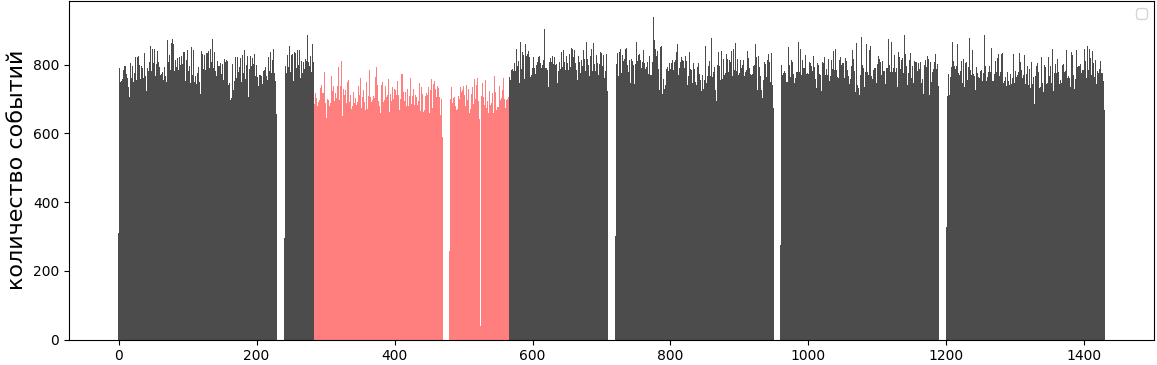
\includegraphics[width=0.9\textwidth, keepaspectratio]{images/19.12.18.png}%
        \label{fig:muon_group1}%
    }%

    \subfloat[]{%
        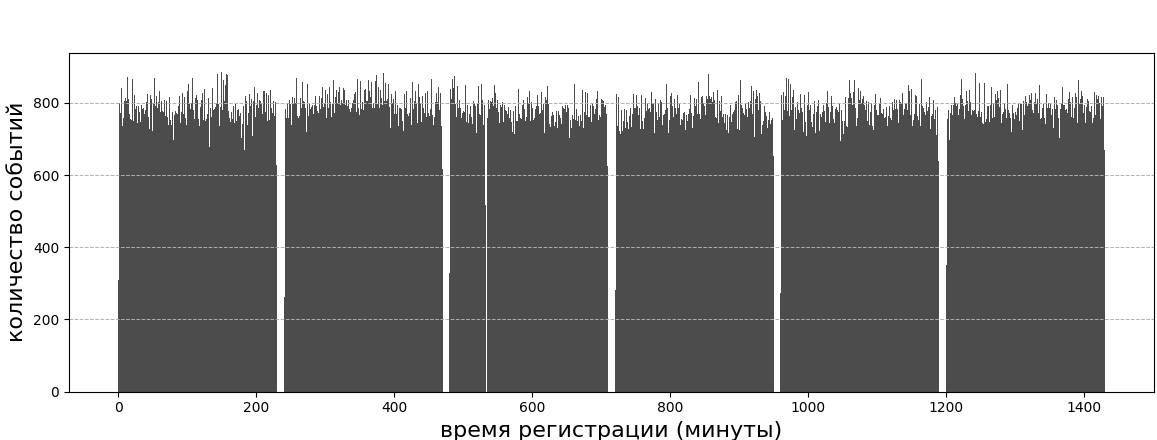
\includegraphics[width=0.9\textwidth, keepaspectratio]{images/20.12.18.png}%
        \label{fig:muon_group}%
    }%

    \caption{Темп счета событий установки НЕВОД-ШАЛ за 19.12.2018 (а) и 20.12.2018 (б)}
    \label{fig:muon_example}
\end{figure}
Можно отметить, что примерно для 20\% событий групп мюонов не было найдено совместных событий на установке НЕВОД-ШАЛ. Для определения причин данного явления был проведен первичный анализ не найденных событий. 

Установка НЕВОД-ШАЛ может работать как в режиме экспозиции, так и мониторинга. Интервалы работы установки в режиме экспозиции разбиваются на временные отрезки длительностью 10 минут, в ходе которых не происходит срабатываний детектирующих станций.
На рисунке 7 представлен темп счета регистрации событий на установке НЕВОД-ШАЛ за 19.12.2018 (а) и 20.12.2018 (б). Видно, что 20.12.2018 (б) установка имеет стабильный в течение всего дня темпы счета, когда за 19.12.2018 (а) имеется резкий спад, что может быть вызвано с временными техническими неисправностями некоторых детектирующий станций. 

Учитывая выше описанные особенности работы установки НЕВОД-ШАЛ, было построено распределение зенитного угла \(\theta\) направлений прихода событий для групп мюонов с отсутствующими совместными событиями на установке НЕВОД-ШАЛ за 19.12.2018 и 20.12.2018 числа (рисунок 8). 

 Из-за меньшей проникающей способности электронно-фотонной компоненты, часть отсутствующих совместных событий установки НЕВОД-ШАЛ можно списать на высокие зенитные углы. 
 \newpage
\begin{figure}[h]
    \centering
    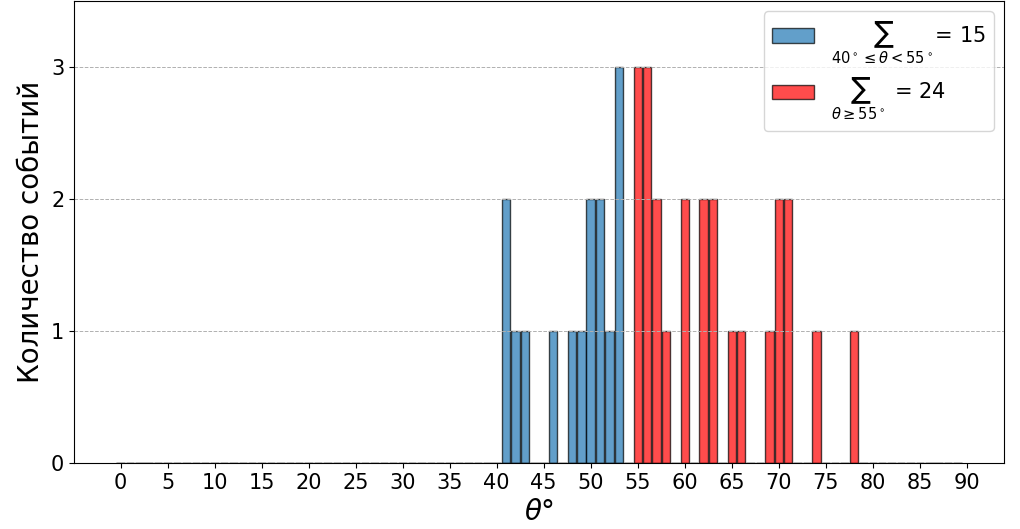
\includegraphics[width=0.85\textwidth]{images/not_events_by_theta.png}
    \caption{Распределение числа событий с группами мюонов без совместного события на установке НЕВОД-ШАЛ по зенитному углу \(\theta\)}
    \label{fig:not_events_by_theta}
\end{figure}
\begin{figure}[h]
    \centering
    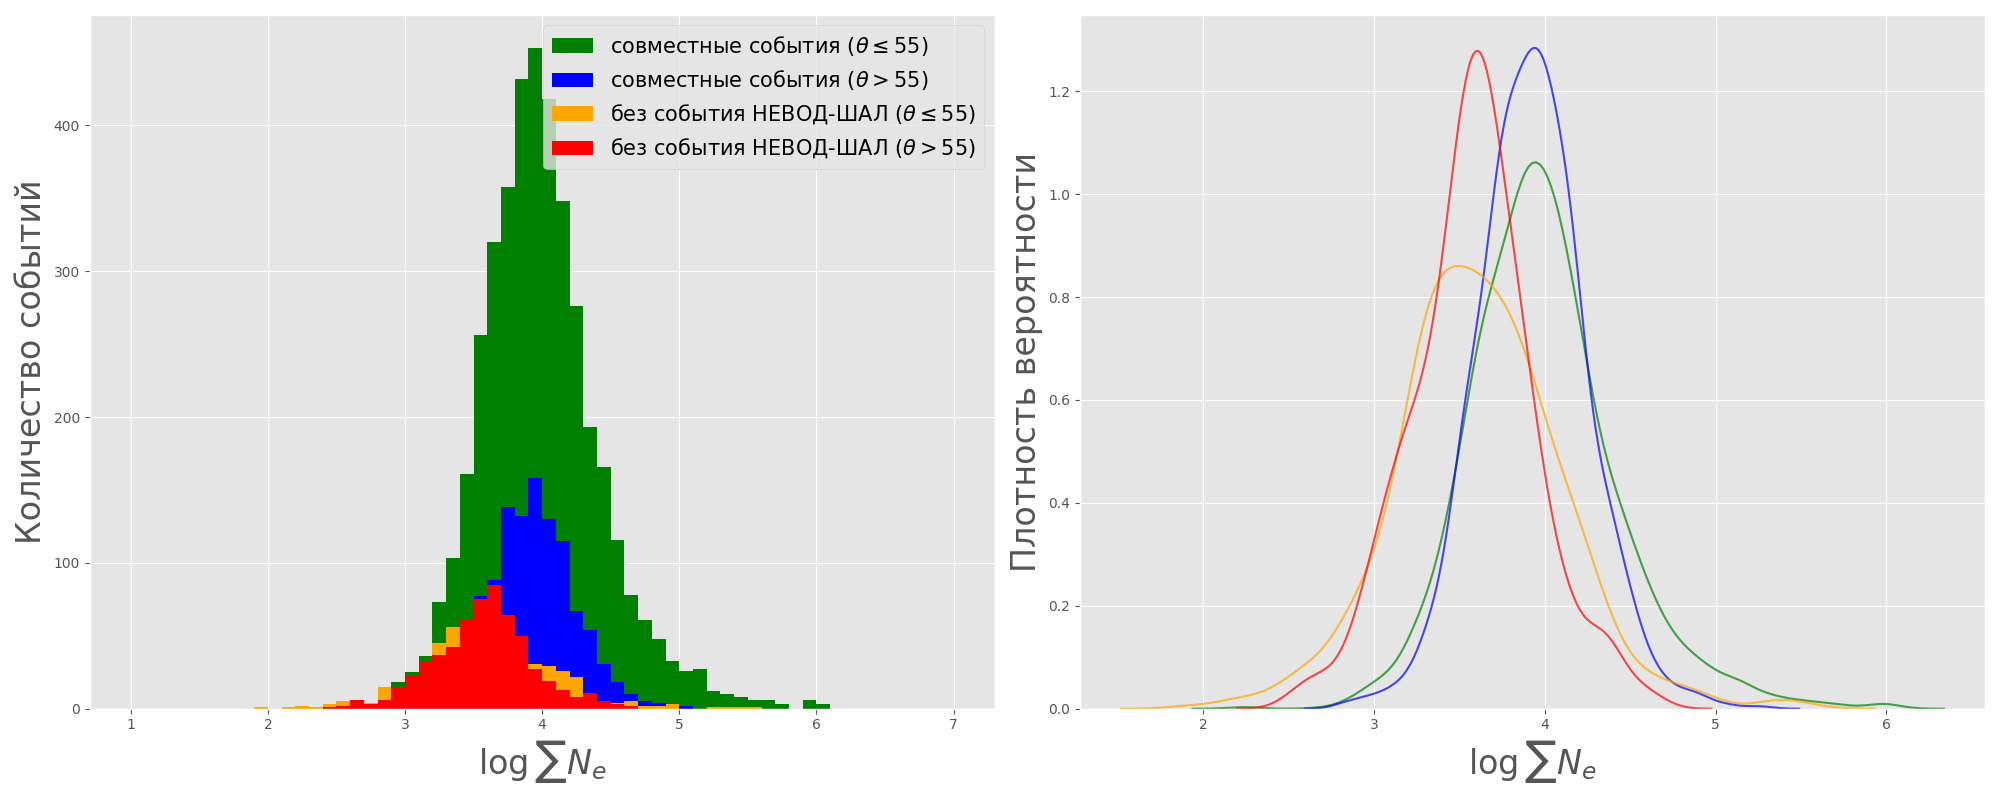
\includegraphics[width=1\textwidth]{images/logQ_theta55.png}
    \caption{Распределения числа событий (слева) и плотности вероятности событий (справа) по десятичному логарифма суммарного сигнала фотоумножителей событий с группами мюонов на ЧВД НЕВОД}
    \label{fig:logQ_theta55}
\end{figure}
\begin{figure}[h]
    \centering
    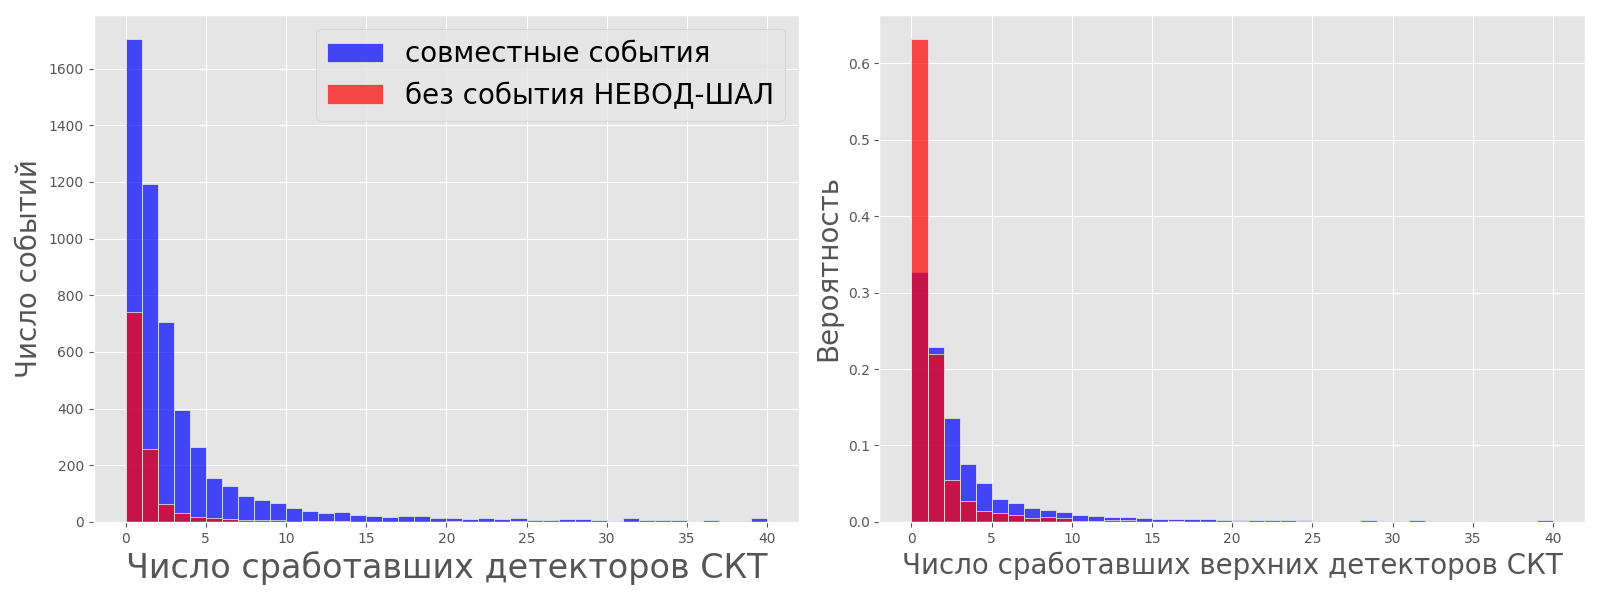
\includegraphics[width=1\textwidth]{images/SKT.png}
    \caption{Распределения числа событий (слева) и плотности вероятности событий (справа) по десятичному логарифма суммарного сигнала фотоумножителей событий с группами мюонов на ЧВД НЕВОД}
    \label{fig:SKT.png}
\end{figure}
\newpage
 
Были рассмотрены отклики на установке ЧВД НЕВОД и детекторах СКТ событий с группами мюонов. На рисунке 9 представлены распределения числа событий (слева) и плотности вероятности событий (справа) по десятичному логарифма суммарного сигнала фотоумножителей событий с группами мюонов на ЧВД НЕВОД.
На рисунке 10 представлены распределения числа событий (слева) и вероятности событий (справа) по числу сработавших верхних детекторов СКТ.
\endinput
                                % поиск совместных событий
\chapter*{Направление прихода ШАЛ}
\addcontentsline{toc}{chapter}{Направление прихода ШАЛ}
\label{ch:intro}

\section*{Кластерный метод реконструкции направления прихода ШАЛ}
\addcontentsline{toc}{section}{Кластерный метод реконструкции направления прихода ШАЛ}
\label{sec:methods}


Направление прихода широкого атмосферного ливня \cite{shulzhenko2019} можно определить по относительным временам срабатывания детектирующих станций установки НЕВОД-ШАЛ, полагая фронт ШАЛ плоскостью, движущейся со скоростью света:
\begin{equation}
Ax+By+Cz+D=0
\end{equation}
уравнение плоскости, где коэффициенты A, B, C  одновременно не равны нулю.
Тогда расстояние между фронтом ШАЛ и детектирующей станцией можно искать, как
расстояние от точки до плоскости:
\begin{equation}
d = \frac{Ax+By+Cz+D}{\sqrt{A^2 + B^2 + C^2}} = ct
\end{equation}
где с - скорость света, t - относительное время срабатываня детектирующей станции.
Если искать вектор направление прихода широкого атмосферного ливня как единичный нормальный вектор, то коэффициенты плоскости нормируются на единицу:
\begin{equation}
A^2 + B^2 + C^2 = 1
\end{equation}
Тогда для поиска коэффициентов плоскости нужно найти минимум функционала:
\begin{equation}
F = \sum_{i=1}^{n} \left(\frac{ct_i - Ax_i - By_i - Cz_i - D}{c} \right)^2
\end{equation}
где n - число всех сработавших детектирующих станций установки невод ШАЛ в одном событии.

Для установки НЕВОД-ШАЛ направление прихода ШАЛ можно определять кластерный методом - усреднение направление прихода события по каждому отдельному сработавшему кластеру. \(t_i\) отсчитываются от момента срабатывания первой детектирующей станции кластера в событии, причем детектируюих станций одного кластера должно быть не менее трех. Зенитный и азимутальный углы \(\theta\) и \(\phi\) направление прихода ШАЛ определяются например как средние или медианное значения соответствующих углов в событии.

Зная, что детектирующие станции одного кластера установки НЕВОД-ШАЛ располагаются примерно на одном уровне, можно преобразовать функционал для кластерного метода к виду:
\begin{equation}
F = \sum_{i=1}^{n} \left(\frac{ct_i - Ax_i - By_i - D}{c} \right)^2
\end{equation}
а значение коэффициента С определяется из условия нормальности направляющего вектора
плоскости фронта широкого атмосферного ливня:
\begin{equation}
C = - \sqrt{1-A^2 - B^2}
\end{equation}

Были построены распределения разницы углов направления прихода ШАЛ совместных событий на установках ДЕКОР и НЕВОД-ШАЛ. Направление прихода события на установку НЕВОЛ-ШАЛ определялось как медианное направлений на сработавшие кластеры. На рисунке 11 представлено распределение \(\Delta \theta = \theta_{\text{Д}} - \theta_{\text{НШ}}\) (а) и распределение \(\Delta \phi = \phi_{\text{Д}} - \phi_{\text{НШ}}\) (б) по числу событий, где
\begin{itemize}
    \item \(\theta_{\text{Д}}, \phi_{\text{Д}}\) зенитный и азимутальный углы направления прихода события на установке ДЕКОР,
    \item \(\theta_{\text{НШ}}, \phi_{\text{НШ}}\) соответственно на НЕВОД-ШАЛ.
\end{itemize}

\begin{figure}[ht]
    \centering
    \subfloat[]{%
        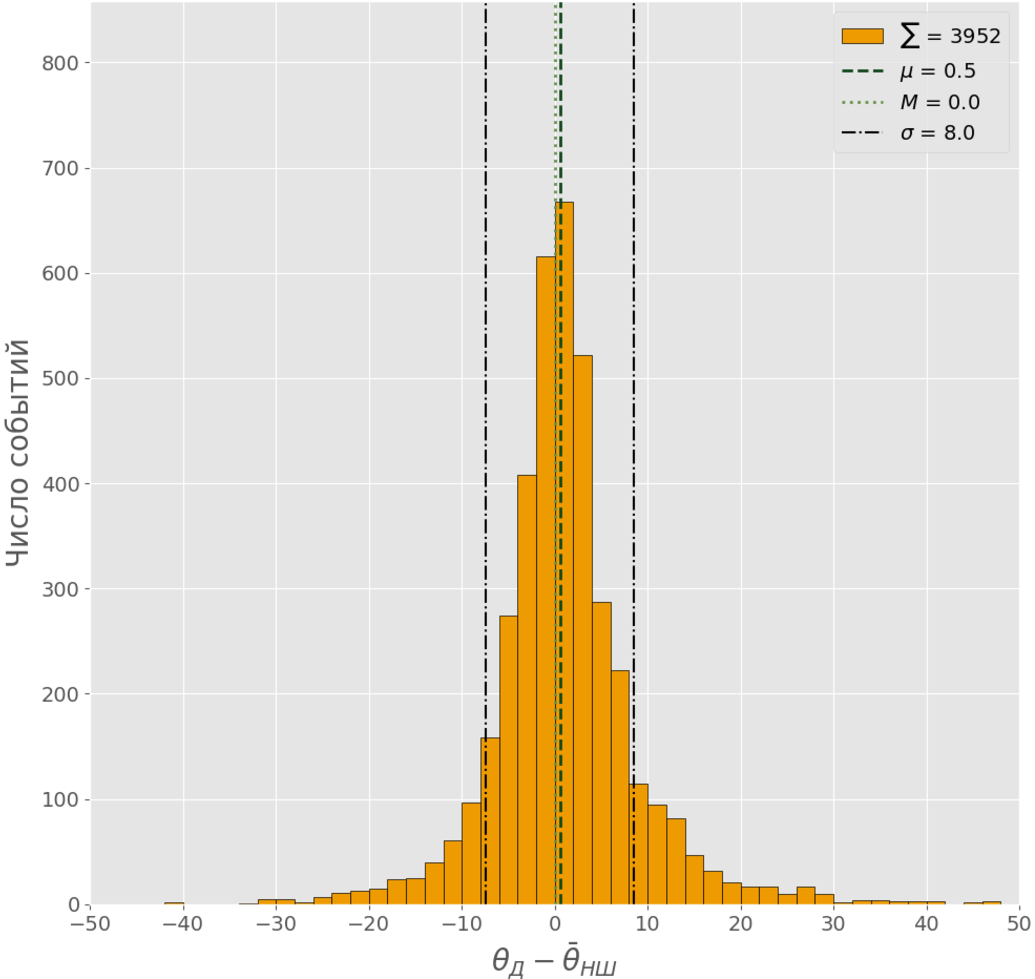
\includegraphics[height=8.5cm, keepaspectratio]{images/theta_hist.png}%
        \label{fig:muon_group1}%
    }%
    \subfloat[]{%
        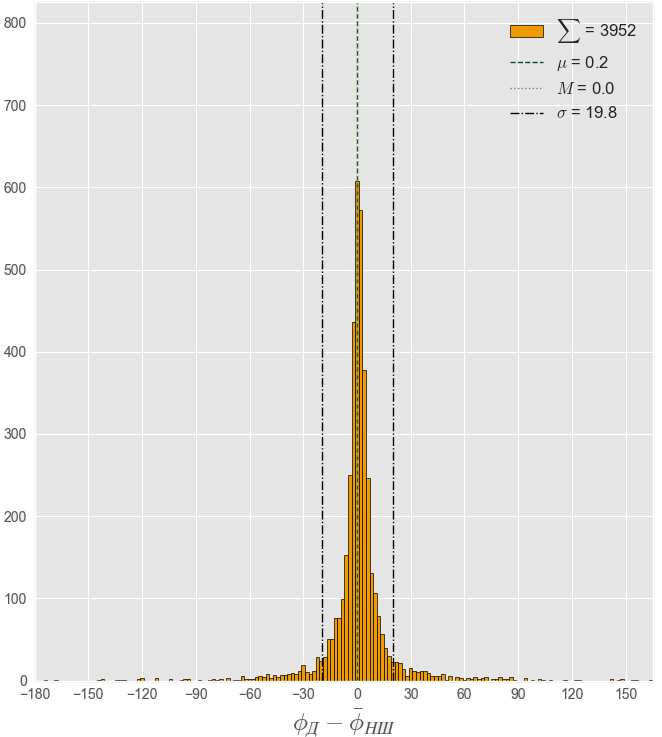
\includegraphics[height=8.5cm, keepaspectratio]{images/phi_hist.png}%
        \label{fig:muon_group}%
    }%

    \caption{распределение числа событий по разности углов направления прихода событий на установках ДЕКОР и НЕВОД-ШАЛ, зенитный угол (а), азимутальный угол (б)}
    \label{fig:muon_example}
\end{figure}


Считая, распределения нормальными можно полагать, что в пределах интервала \(\sigma_{\theta}\) = \(8\degree\) \((−\sigma_{\theta},+\sigma_{\theta})\) (где \(\sigma_{\theta}\) — стандартное отклонение) у 68\% событий зенитный угол \(\theta\) различается незначительно. Азимутальные углы имеют большее стандартное отклонение  \(\sigma_{\phi} = 20\degree\ \).

Большие выбросы на хвостах распределений объясняются низким числом сработавших кластеров НЕВОД-ШАЛ. На рисунке 12 представлено распределение угла между векторами направлений прихода событий ДЕКОР и НЕВОД-ШАЛ \(\angle(\mathbf{n_{\text{Д}}}, \mathbf{n_{\text{НШ}}})\)

\begin{figure}[ht]
    \centering
    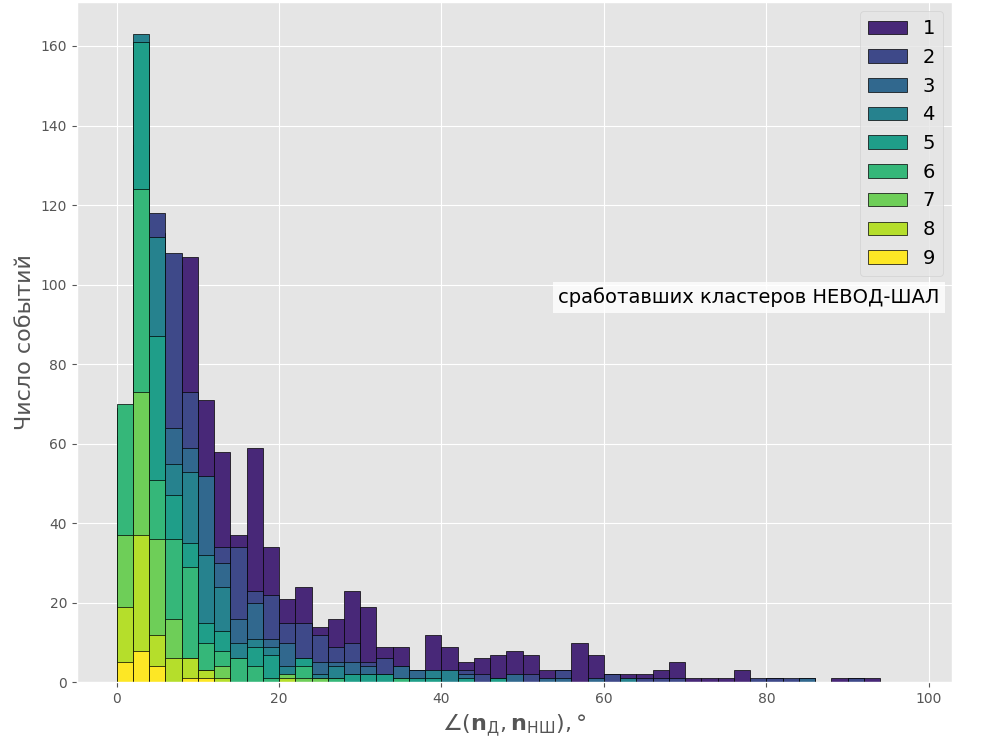
\includegraphics[width=1\textwidth]{images/vecs_angel.png}
    \caption{распределение числа событий по углу между векторами направления прихода событий на установках ДЕКОР и НЕВОД-ШАЛ}
    \label{fig:vecs_angel}
\end{figure}


Из распределения видно, что определение направления прихода события на НЕВОД-ШАЛ сходится к направлению на ДЕКОР при росте числа сработавших кластеров.

\section*{Вероятностная постановка задачи реконструкции}
\addcontentsline{toc}{section}{Вероятностная постановка задачи реконструкции}
\label{sec:methods}
Введу некоторые определения.
Пусть задано множество объектов \(X\), множество допустимых ответов \(Y\), и существует целевая функция \(\tilde{y} : X \to Y\), значения которой \(y = \tilde{y}(x_i)\) известны только на конечном подмножестве объектов \(\{x_1,...,x_l\} \subset X\). Задача обучения по парам \((x_i, y_i)\) заключается в том, чтобы по выборке \(X^l\) восстановить зависимость \(\tilde{y}\), то есть построить решающую функцию \(a : X \to Y\) , которая приближала бы целевую функцию \(\tilde{y}\), причём не только на  \(\{x_1,...,x_l\}\), но и на всём множестве X.

Решающая функция \(a\) должна допускать эффективную компьютерную реализацию, по этой причине буду называть её алгоритмом.

Признаком \(f\) объекта \(x\) будет результат измерения некоторой характеристики объекта. Формально признаком называется отображение \(f : X \to D_f\) , где \(D_f\)
множество допустимых значений признака.

В задаче реконструкции направления прихода ШАЛ в роли объектов выступят совместные события на установках. Признаки могут характеризовать координаты ДС, времена срабатываний ДС, задержки срабатывания ДС, положения мюонных пиков ДС, темпы счета ДС за определенный период и так далее, а в роли ответов выступают направления прихода событий ШАЛ.

Данные могут быть неточными, поскольку измерения значений признаков \(f_j(x)\) и целевой зависимости \(\tilde{y}\) обычно выполняются с погрешностями. Данные могут быть неполными, поскольку измеряются не все мыслимые признаки, а лишь физически доступные для измерения или например измерение времени срабатываний ДС может просто отсутствовать, если станция не сработала. В таком случае \(\tilde{y}\), строго говоря, не является функцией. Можно попробовать устранить эту некорректность с помощью вероятностной постановки задачи.

Вместо существования неизвестной целевой зависимости \(\tilde{y}\) предположим существование неизвестного вероятностного распределения на множестве \(X \times Y\)
с плотностью \(p(x, y)\), из которого случайно и независимо выбираются \(l\) наблюдений
\(X^l = (x_i, y_i)^{l}_{i=1}\). Такие выборки называются простыми.

Вероятностная постановка задачи считается более общей, так как функциональную зависимость \(\tilde{y}\) можно представить в виде вероятностного распределения \(p(x, y) = p(x)p(y|x)\), положив \(p(y|x) = \delta(y - \tilde{y})\), где \(\delta(z)\) - дельта-функция.

При вероятностной постановке задачи задаётся модель совместной плотности распределения объектов и ответов \(\xi(x, y, w)\), аппроксимирующая неизвестную плотность \(p(x, y)\). Затем определяется значение параметра \(w\), при котором выборка данных \(X_l\) максимально правдоподобна, то есть наилучшим образом согласуется с моделью плотности. Если наблюдения в выборке \(X_l\) независимы, то совместная плотность распределения всех наблюдений равна произведению плотностей \(p(x, y)\) в каждом наблюдении: \(p(X_l) = p((x_1,y_1, ..., x_l, y_l))= p(x_1,y_1) \cdot ... \cdot p(x_l,y_l)\). Подставляя вместо \(p(x, y)\) модель плотности \(\xi(x, y, w)\), получаем функцию правдоподобия
\begin{equation}
L(w, X^l) = \prod_{i=1}^l \xi(x_i,y_i,w)
\end{equation}
Чем выше значение правдоподобия, тем лучше выборка согласуется с моделью. Значит, нужно искать значение параметра \(w\), при котором значение \(L(w, X^l)\) максимально - принципом максимума правдоподобия.

Вместо максимизации \(L\) удобнее минимизировать функционал − \(\ln{L}\), поскольку
он имеет вид суммы:
\begin{equation}
-\ln{L(w, X^l) = - \sum_{i=1}^l \ln{\xi(x_i,y_i,w)} \to min}
\end{equation}
Пусть задана модель \(a(x, w)\), примем дополнительное вероятностное предположение,
что ошибки \( \varepsilon(x, w) = a(x, w) - \tilde{y}\) имеют нормальное распределение 
\(N(\varepsilon, 0, \sigma^2) = \frac{1}{\sigma \sqrt{2\pi}}\exp(-\frac{\varepsilon^2}{2\sigma^2})\) с нулевым средним и дисперсией \(\sigma^2\). Тогда модель плотности имеет вид
\begin{equation}
\xi(x,y,w) = p(x)\xi(y|x,w) = p(x)N(a(x, w) - \tilde{y};0,\sigma^2)
\end{equation}
Отсюда следует, что вероятностная функция потерь совпадает с квадратичной с точностью до констант \(C_0\) и \(C_1\), не зависящих от параметра \(w\)
\begin{equation}
-\ln{\xi(x,y,w)} = - \ln{p(x)N(a(x,w) - \tilde{y}(x);0,\sigma^2)} = C_0 + C_1(a(x,w) - \tilde{y}(x))^2
\end{equation}
Постоянными слагаемыми можно пренебречь тогда оказывается, что максимизация функции правдоподобия равносильна минимизации
\begin{equation}
\sum_{i=1}^l(\tilde{y}(x_i) - a(x_i, w))^2
\end{equation}
получилась неотрицательная функция, характеризующая величину реднеквадратичной ошибки алгоритма \(a\) на объекте \(x\).

Для построения решающей функции буду использовать многослойную нейронная сеть -  сложную дифференцируемуя функцию, задающая отображение из исходного признакового пространства в пространство ответов, все параметры которой могут настраиваться одновременно и взаимосвязанно. Многослойные сети можно настраивать градиентными методами, несмотря на огромное количество весовых коэффициентов. Хотя количество операций, необходимых для вычисления градиента, обычно возрастает пропорционально размерности, то есть числу весовых коэффициентов, этого удаётся избежать благодаря аналитическому дифференцированию суперпозиции с сохранением необходимых промежуточных величин - методу обратного распространения ошибок \cite{lecun1988theoretical}.

Рассмотрю многослойную сеть, в который каждый нейрон предыдущего слоя
связан со всеми нейронами последующего слоя. Введу следующие обозначения. Пусть выходной слой состоит из \(M\) нейронов с функциями активации \(\sigma_m\) и выходами (ответами) \(a^m\), \(m=1,...,M\). Перед ним находится скрытый слой из \(H\) нейронов с функциями активации \(\sigma_h\) и и выходами \(u_h\), \(h=1,...,H\). Веса cвязей между \(h\)-м нейроном скрытого слоя и \(m\)-м нейроном выходного слоя будем обозначать через \(w_{hm}\). Перед этим слоем может находиться либо входной слой признаков, либо ещё один скрытый слой с выходами \(v^j\), \(j=1,...,J\) и весами \(w_{jh}\). В общем случае число слоёв может быть произвольным. Если сеть двухслойная, то \(v^j\) есть просто \(j\)-й признак: \(v^j(x)=f_j(x)=x^j\), и \(j=n\). Обозначу через \(w\) вектор всех весов сети. Пример многослойной сети с одним скрытым слоем представлен на рисунке 13. 
\begin{figure}[ht]
    \centering
    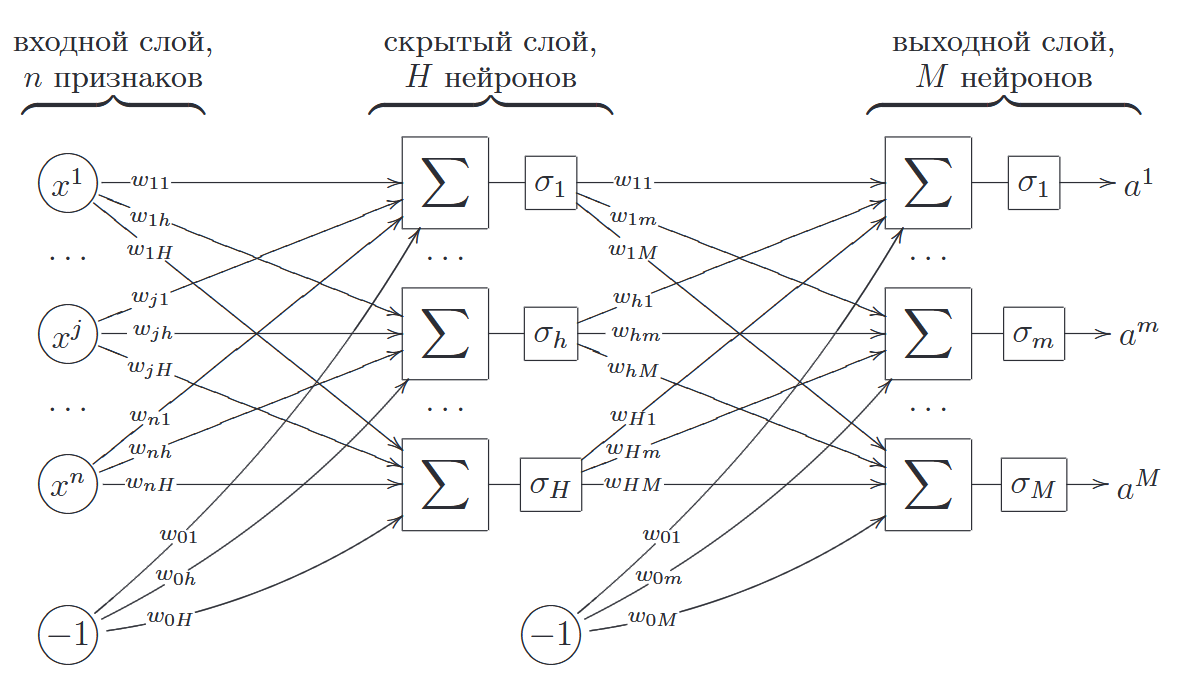
\includegraphics[width=1\textwidth]{images/nn.png}
    \caption{Многослойная сеть}
    \label{fig:nn}
\end{figure}

Выходные значения сети на \(x_i\) вычисляются как суперпозиция:
\begin{equation}
a^m(x_i) = \sigma_m \left(\sum_{h=0}^H w_{hm} u^h(x_i) \right); \qquad
u^h(x_i) = \sigma_h \left(\sum_{j=0}^J w_{jh} v^j(x_i) \right)
\end{equation}

Зафиксирую \(x_i\) и запишу функцию среднеквадратичной ошибки
\begin{equation}
Q(w) = \frac{1}{2}\sum_{m=1}^M \left(a^m(x_i) - y^m_i \right)^2
\end{equation}
Частная производная \(Q\) по выходам нейронов выходного слоя:
\[
\frac{\partial Q(w)}{\partial a^m} = a^m(x_i) - y^m_i = \varepsilon^m_i
\]
Частная производная \(Q\) по \(a_m\) равна величине ошибки \(\varepsilon^m_i\) на \(x_i\). Частные производные по выходам скрытого слоя:
\[
\frac{\partial Q(w)}{\partial u^h} = \sum_{m=1}^M \left(a^m(x_i) - y^m_i \right)\sigma'_m w_{hm} = \sum_{m=1}^M \varepsilon^m_i \sigma'_m w_{hm} = \varepsilon^h_i
\]
Получается ошибка сети на скрытом слое \(\varepsilon^h_i\). \(\varepsilon^h_i\) вычисляется по \(\varepsilon^m_i\), если запустить сеть «задом наперёд», подав на выходы нейронов скрытого слоя значения \(\varepsilon^m_i \sigma'_m\), а результат \(\varepsilon^h\) получив на входе. При этом входной вектор скалярно умножается на вектор весов \(w_{hm}\), находящихся справа от нейрона, а не слева, как при прямом вычислении 

\begin{minipage}{0.4\textwidth}
  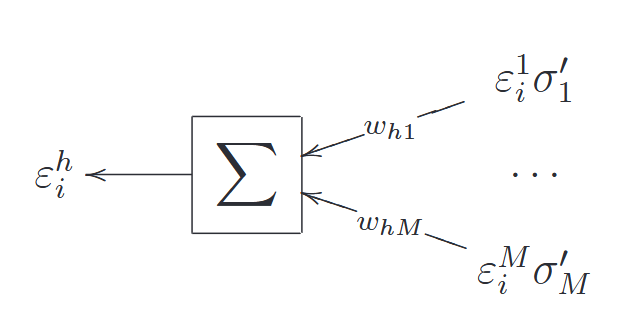
\includegraphics[width=\textwidth]{images/nn1.png}
\end{minipage}
\par
Градиент \(Q\) по весам:
\begin{equation}
\frac{\partial Q(w)}{\partial w_{hm}} = \frac{\partial Q(w)}{\partial a^m}  \frac{\partial a^m)}{\partial w_{hm}} = \varepsilon^m_i \sigma'_m u^h(x_i), \qquad m=1,...,M, \quad h=0,...,H;
\end{equation}
\begin{equation}
\frac{\partial Q(w)}{\partial w_{jh}} = \frac{\partial Q(w)}{\partial u^h}  \frac{\partial u^h)}{\partial w_{jh}} = \varepsilon^h_i \sigma'_h v^j(x_i), \qquad h=1,...,H, \quad j=0,...,J;
\end{equation}
и так далее для каждого слоя. Если слоёв больше двух, то остальные частные производные вычисляются аналогично - обратным ходом по слоям сети справа налево.

С помощью нейросети легко создать модель, которая предсказывает сразу и зенитный \(\theta\), и азимутальный \(\phi\) угол направления прихода ШАЛ. Достаточно сделать, чтобы последнее представление было матрицей \(B \times M\), где \(B\) - число объектов, а \(M\) — количество предсказываемых чисел. И тогда можно минимизировать фунцию по всей матрице \(B \times M\).

Для проверки работы модели были рассчитаны относительные времена срабатывания  детектирующих станций установки НЕВОД-ШАЛ для заданных углов направления прихода событий \(\theta \in [0,\frac{\pi}{2}]\), \(\phi \in [0, 2\pi)\) - пусть в момент времени \(t=0\) соответствует положению фронта, когда он проходит через начало координат \(\textbf{r}=[0,0,0]\), для ДС, время срабатывания определяется относительно этого момента как 
\(t_i = - \frac{\mathbf{r}_i \cdot \mathbf{v}}{c}\), где 
\begin{itemize}
    \item \(\mathbf{r_i}\) радиус-вектор к ДС,
    \item \(\mathbf{v} = [\sin{\theta}\cos{\phi}, \sin{\theta}\sin{\phi}, \cos{\theta}]\) вектор направления прихода ШАЛ,
    \item \(c\) скорость света.
\end{itemize}

Для приближения соответствия данных к реальным наблюдаемым событиям на установке НЕВОД-ШАЛ учтено, что не все детектирующие станции могут срабатывать. На рисунке 14 представлено распределение разницы предсказаний модели и заданных значений углов \(\theta\) и \(\phi\) для 7080 разыгранных событий, не участвующих в построении решающей функции.
\begin{figure}[ht]
    \centering
    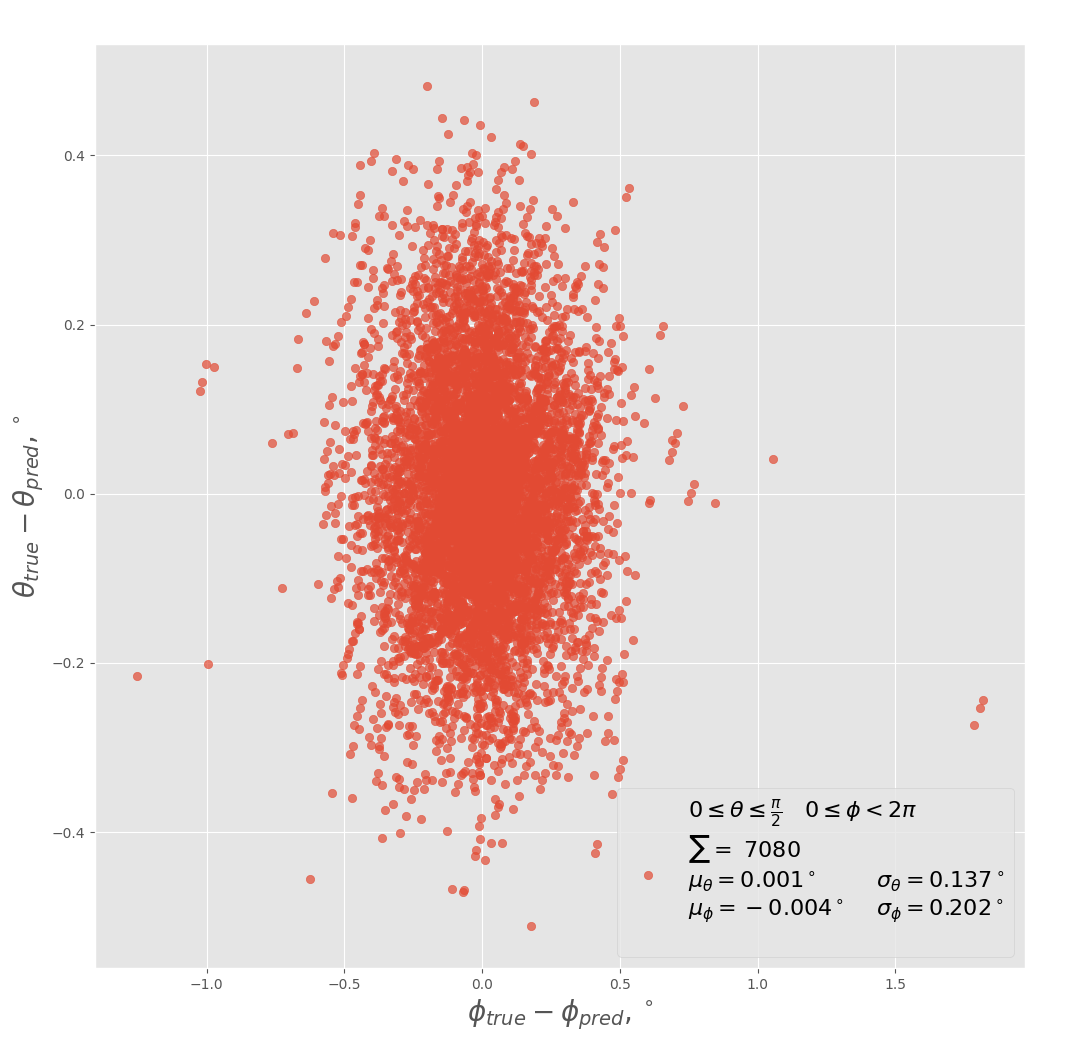
\includegraphics[width=0.95\textwidth]{images/test_theta_vs_phi_diff.png}
    \caption{Распределение разницы предсказаний модели и заданных значений углов \(\theta\) и \(\phi\) направлений прихода ШАЛ}
    \label{fig:nn}
\end{figure}

Для предсказания значений \(\theta\) и \(\phi\) найденных совместных событий на установках ДЕКОР и НЕВОД-ШАЛ были создан синтетический набор данных откликов ДС. Для учета задержек срабатывания ДС и влияние системных и статистических факторов на результаты измерений был добавлен шум, соответствующий значениям распределения разницы времени откликов, вычисленных по направлению прихода совместного события на установку ДЕКОР, и реальным временем срабатывания ДС установки НЕВОД-ШАЛ для того же события. На рисунке 15 и 16 представлены значения зенитного угла \(\theta\) и \(\phi\) найденных совместных событий, определенные по данным установки ДЕКОР, НЕВОД-ШАЛ и моделью. 
\begin{figure}[ht]
    \centering
    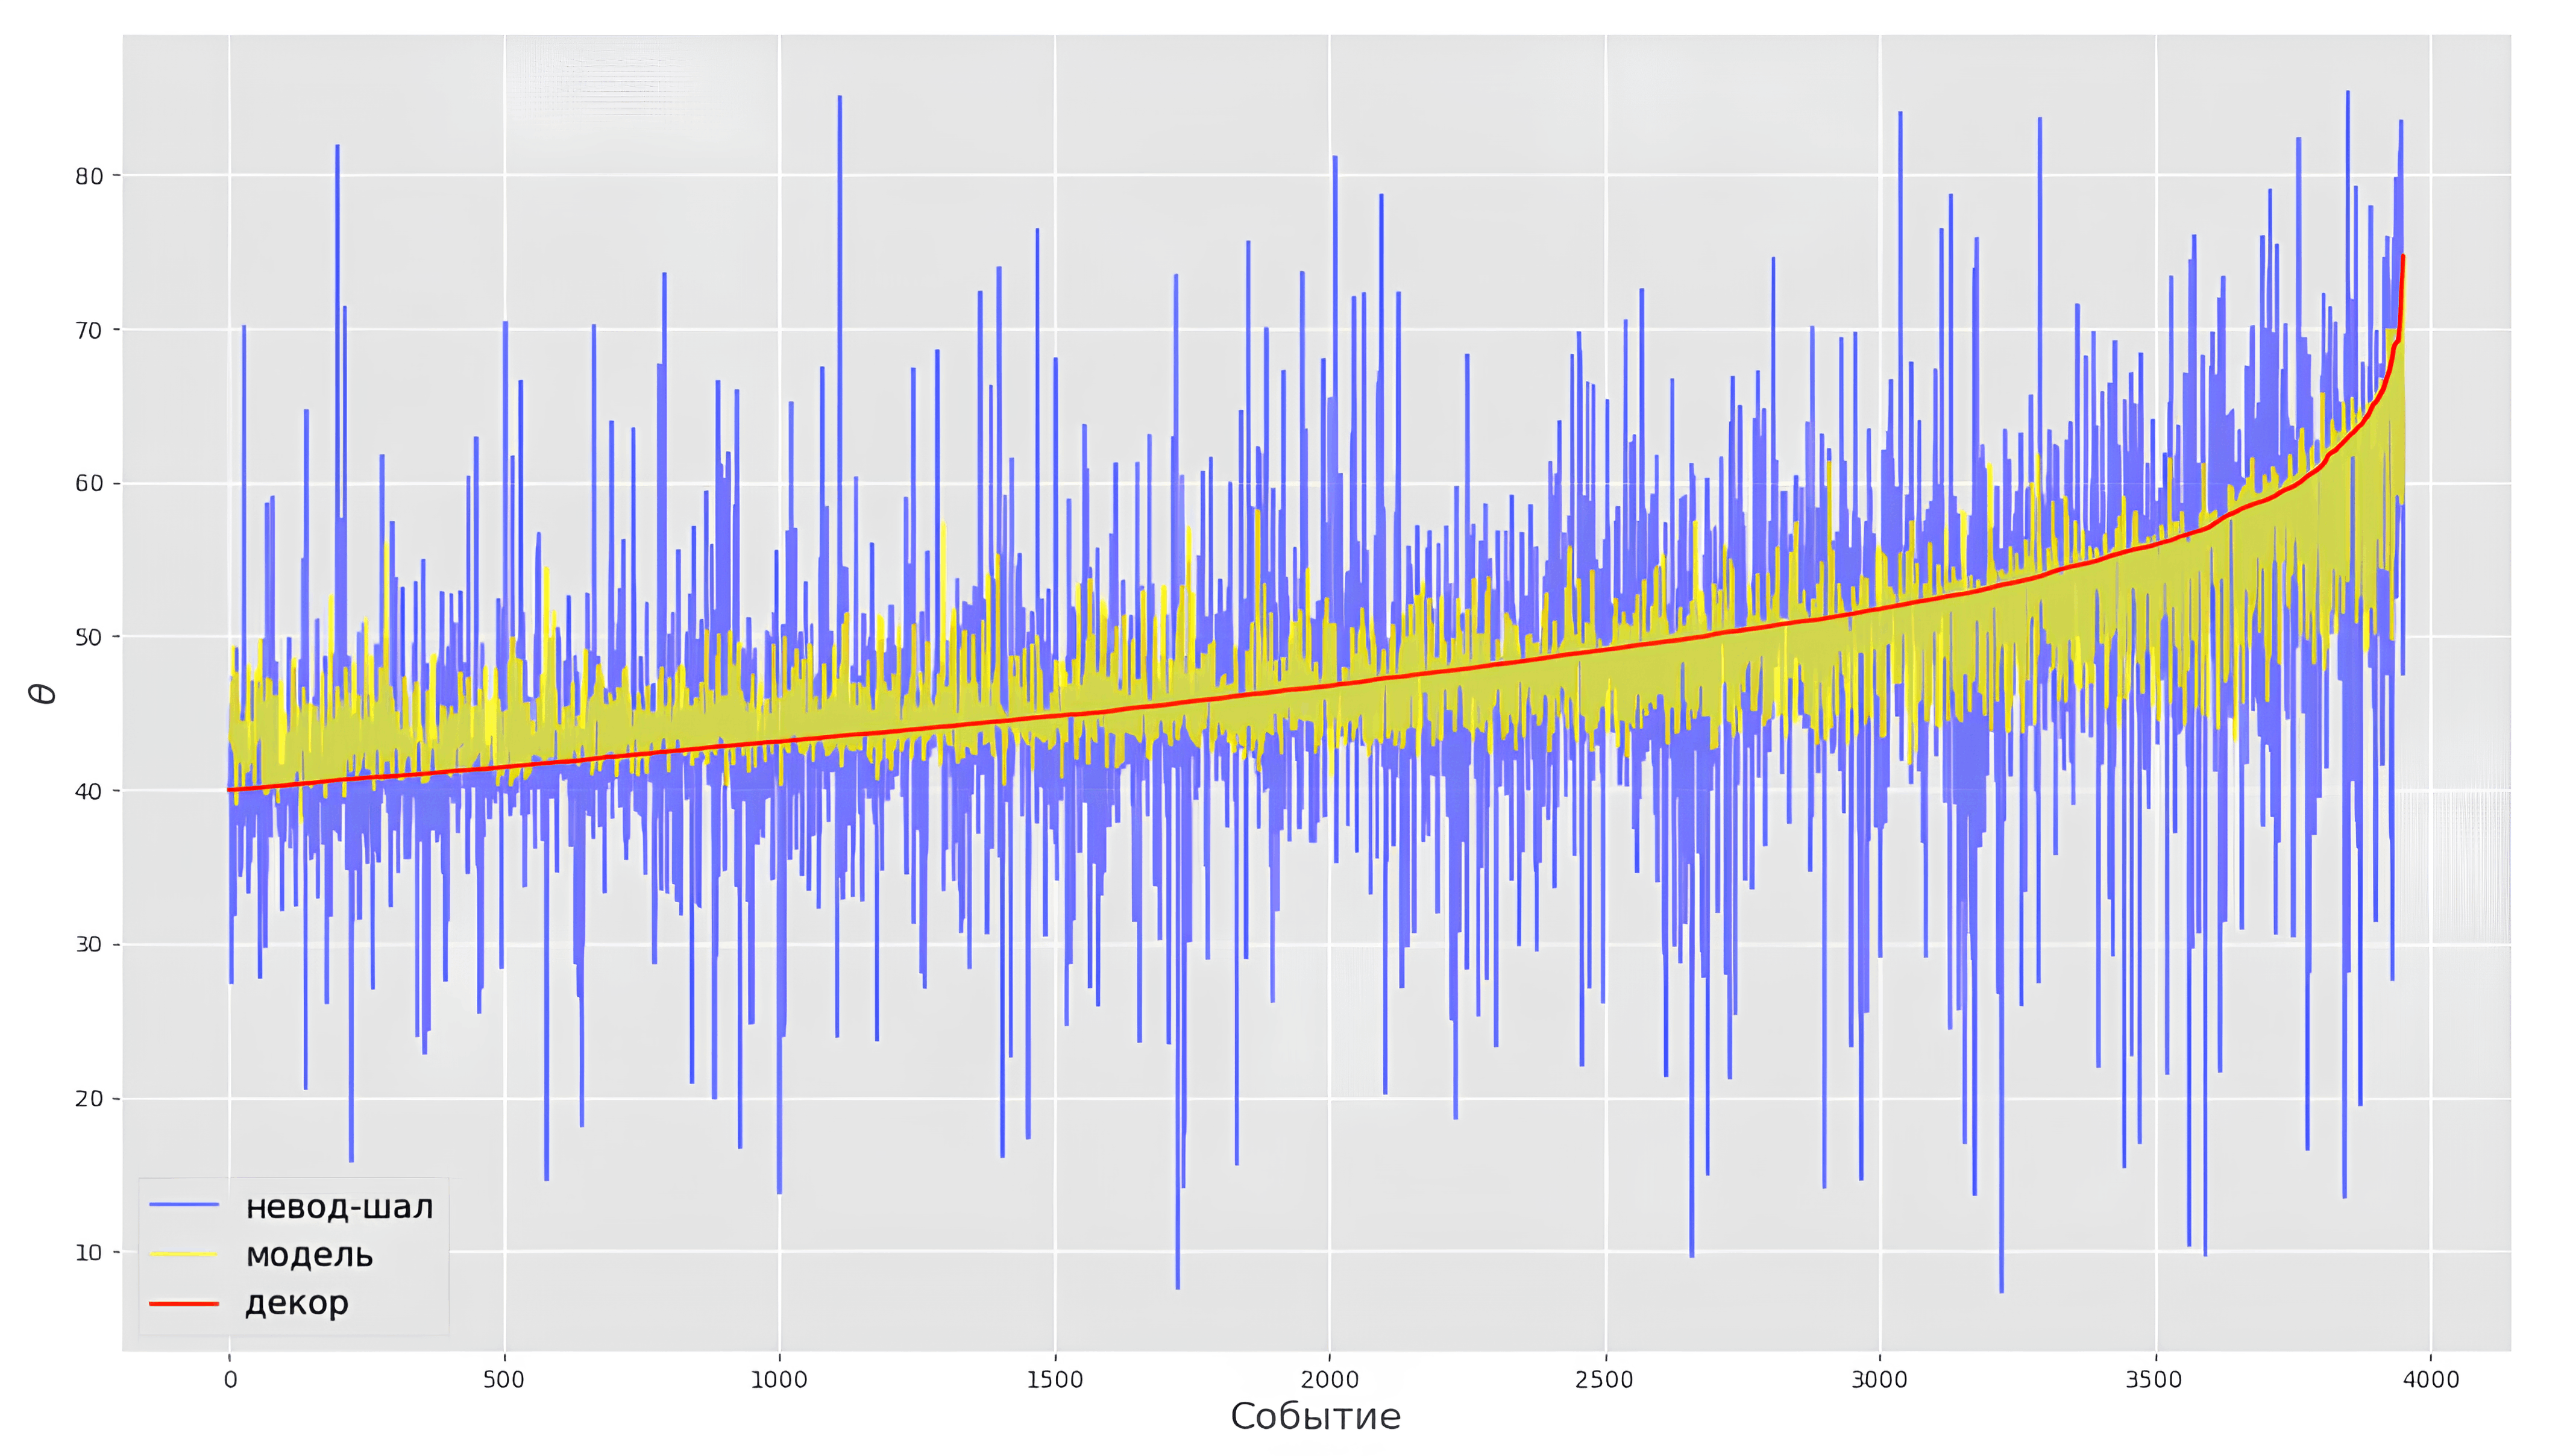
\includegraphics[width=1\textwidth]{images/theta_3_1.png}
    \caption{Значения зенитного угла \(\theta\) найденных совместных событий, определенные по данным установки ДЕКОР (красный), НЕВОД-ШАЛ (синий) и моделью (желтый)}
    \label{fig:theta}
\end{figure}

\begin{figure}[ht]
    \centering
    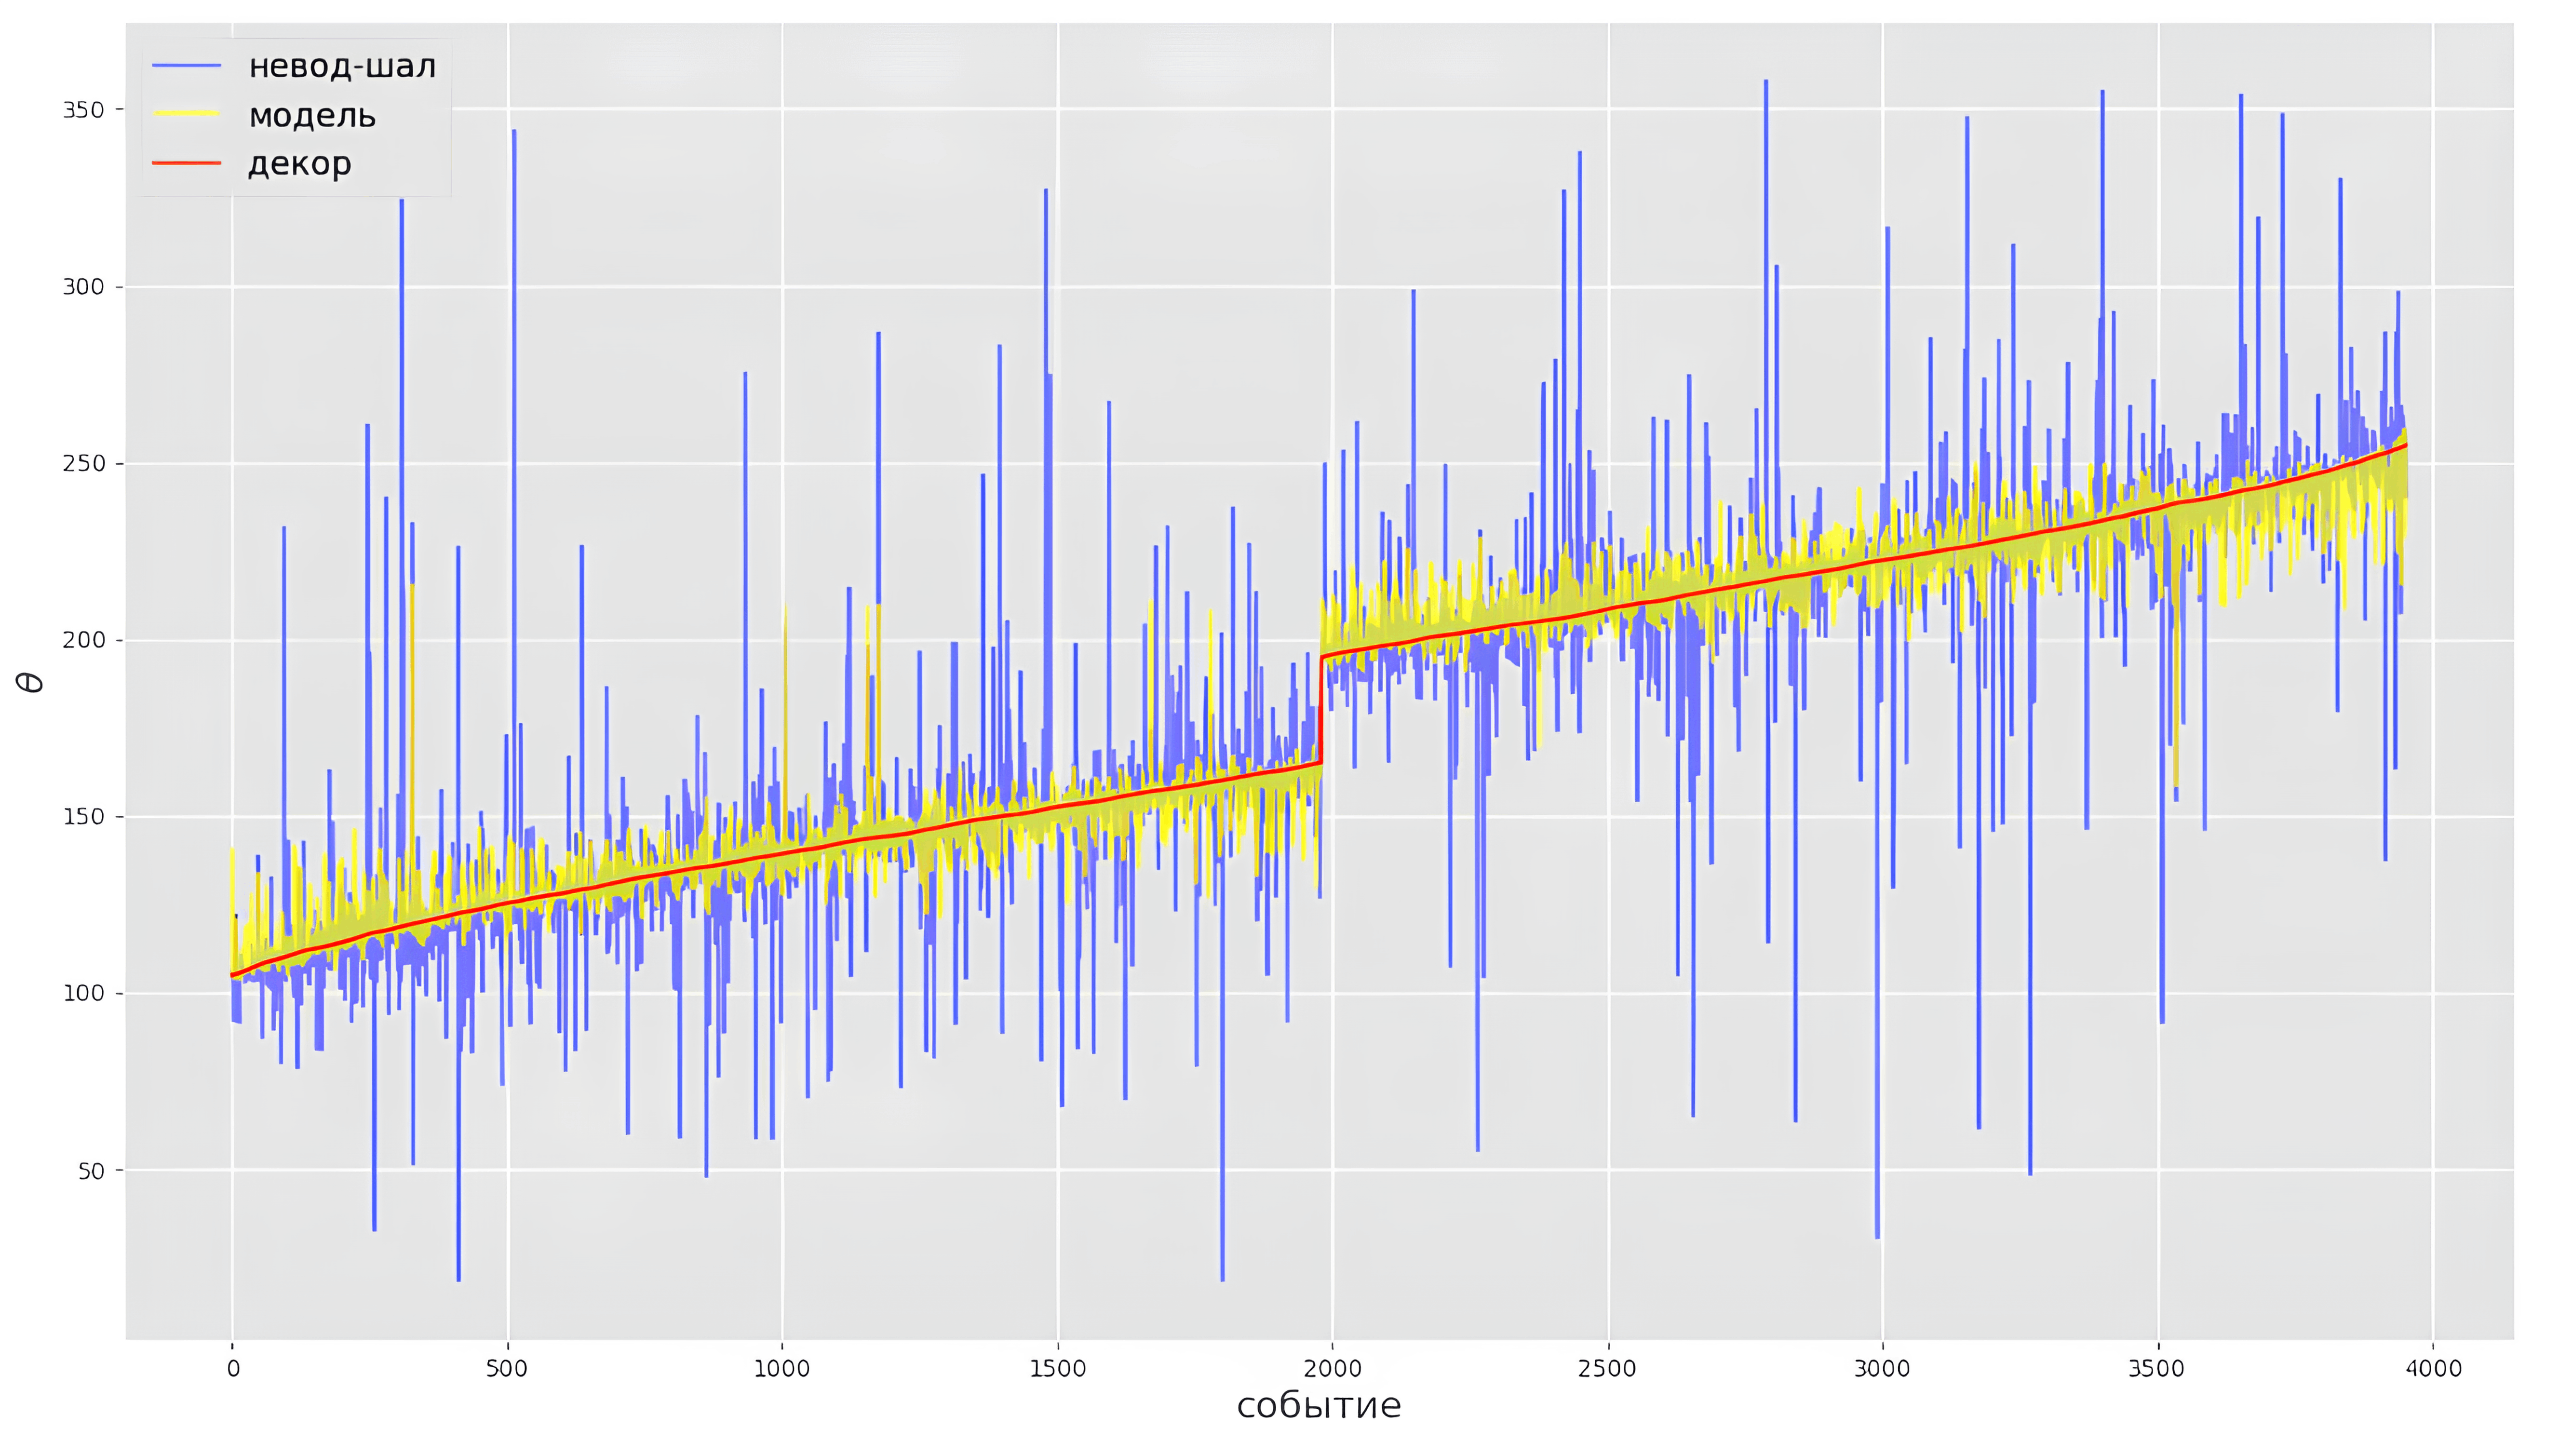
\includegraphics[width=1\textwidth]{images/phi_3_1.png}
    \caption{Значения азимутального угла \(\phi\) найденных совместных событий, определенные по данным установки ДЕКОР (красный), НЕВОД-ШАЛ (синий) и моделью (желтый)}
    \label{fig:phi}
\end{figure}

\clearpage 
Квадратичный корень из средней квадратичной ошибки предсказаний модели и значениями ДЕКОР:
\[
RMSE = \sqrt{\frac{1}{N}\sum_{i=1}^N \| \mathbf{y_{\text{Д}}} - \mathbf{y_{\text{М}}} \|^2} = 5.8 \degree
\]
Для сравнения квадратичный корень из средне квадратичного расхождения значений ДЕКОР и НЕВОД-ШАЛ равен \(20.9\degree\).

Учитывая, что сходимость направления прихода события на установке НЕВОД-ШАЛ к направлению прихода совместного события на установке ДЕКОР пропорциональна числу сработавших кластеров на НЕВОД-ШАЛ, можно обучать модель непосредственно на значениях направления прихода совместного события на установке ДЕКОР. В теоретическом плане, с увеличением объема выборки совместных событий на установках, а также с учетом регистрации групп мюонов, приходящих под любыми углами, возможно более точное реконструирование направления любого события, зарегистрированного установкой НЕВОД-ШАЛ. 
\endinput                             % направление прихода
\chapter*{Заключение}
\addcontentsline{toc}{chapter}{Заключение}
\label{ch:intro}

В ходе выполнения научно-исследовательской работы были решены следующие задачи:
\begin{itemize}
    \item поиск совместных событий на установке НЕВОД-ШАЛ для событий с группами мюонов на установке ДЕКОР за период с 19.12.2018 по 02.02.2019,
    \item рассмотрение откликов установки ЧВД НЕВОД и детекторов СКТ с не найденными совместными событиями на установке НЕВОД-ШАЛ для событий  с группами мюонов на установке ДЕКОР,
    \item разработан, обучен и протестирован искусственный нейронный сетевой алгоритм для реконструкции направлений прихода широкого атмосферного ливня,
    \item Восстановление направлений прихода совместных событий на установке НЕВО-ШАЛ с квадратичным корнем из средне квадратичного расхождением \(5.8 \degree\) с реконструкцией на установке ДЕКОР.
\end{itemize}

В результате проведенной работы предсказаны направления прихода найденных совместных событий ШАЛ. Построены сравнительные распределения зенитного и азимутального углов направлениях прихода событий. 




\endinput 
\printbibliography[title=Список использованных источников] 
%%\input{3_chap1}                                     % Первая глава
%%\input{4_chap2}                                     % Вторая глава
%%\input{5_chap3}                                     % Третья глава


\end{document}